%%%%%% -*- Coding: utf-8-unix; Mode: latex

%\documentclass[polish]{projectreport}
\documentclass[english]{projectreport}

\usepackage[utf8]{inputenc}
\usepackage{url}
\usepackage{subfigure}
\usepackage{tabularx}
\usepackage{ragged2e}
\usepackage{booktabs}
\usepackage{multirow}
\usepackage{grffile}

\usepackage[bookmarks=false]{hyperref}
\hypersetup{colorlinks,
  linkcolor=blue,
  citecolor=blue,
  urlcolor=blue}

\usepackage{indentfirst}
\usepackage{caption}
\usepackage{listings}
\usepackage[ruled,linesnumbered,lined]{algorithm2e}
\usepackage[svgnames]{xcolor}
\usepackage{inconsolata}
\usepackage{fancyhdr}

\usepackage{minted} % for JSON code snippets

\usepackage{subcaption}

\usepackage{hyperref}

\usepackage{csquotes}
\DeclareQuoteStyle[quotes]{polish}
  {\quotedblbase}
  {\textquotedblright}
  [0.05em]
  {\quotesinglbase}
  {\fixligatures\textquoteright}
\DeclareQuoteAlias[quotes]{polish}{polish}

\usepackage[
style=numeric,
sorting=nyt,
isbn=false,
doi=true,
url=true,
backref=false,
backrefstyle=none,
maxnames=10,
giveninits=true,
abbreviate=true,
defernumbers=false,
backend=biber]{biblatex}
\addbibresource{bibliography.bib}

\lstset{
    % language=JSON, %% PHP, C, Java, etc.
    basicstyle=\ttfamily\footnotesize,
    backgroundcolor=\color{gray!5},
    commentstyle=\it\color{Green},
    keywordstyle=\color{Red},
    stringstyle=\color{Blue},
    numberstyle=\tiny\color{Black},    
    % morekeywords={TestKeyword},
    % mathescape=true,
    escapeinside=`',
    frame=single, %shadowbox, 
    tabsize=2,
    rulecolor=\color{black!30},
    title=\lstname,
    breaklines=true,
    breakatwhitespace=true,
    framextopmargin=2pt,
    framexbottommargin=2pt,
    extendedchars=false,
    captionpos=b,
    abovecaptionskip=5pt,
    keepspaces=true,            
    numbers=left,                    
    numbersep=5pt,                  
    showspaces=false,                
    showstringspaces=false,
    showtabs=false,
    tabsize=2
}

\SetAlgorithmName{\LangAlgorithm}{\LangAlgorithmRef}{\LangListOfAlgorithms}

\renewcommand{\lstlistingname}{\LangListing}
\renewcommand\lstlistlistingname{\LangListOfListings}

\newcolumntype{Y}{>{\small\centering\arraybackslash}X}
%\newcolumntype{b}{>{\hsize=1.6\hsize}Y}
%\newcolumntype{m}{>{\hsize=.6\hsize}Y}
%\newcolumntype{s}{>{\hsize=.4\hsize}Y}

\captionsetup[figure]{skip=5pt,position=bottom}
\captionsetup[table]{skip=5pt,position=top}



%%%%%%%%%%%%%%%%%%%%%%%%%%%%%%%%%%%%%%%%%%%%%%%%%%%%%%%%%%%%%%%%%%%%%%%%%%%%%%%
\author{Kacper Cienkosz$^1$ \and Miłosz Dubiel$^2$}

\title{The multi-agent based socio-economical simulation}

\date{
	{\small $^1$AGH University of Krakow \\ \texttt{kcienkosz@student.agh.edu.pl}\\[1ex]%
	$^2$AGH University of Krakow \\ \texttt{miloszdubiel@student.agh.edu.pl}\\[2ex]%
        \the\year}
      }
      
\pagestyle{fancy}
\fancyhf{}
\fancyhead[LE,RO]{\thepage}

%%%%%%%%%%%%%%%%%%%%%%%%%%%%%%%%%%%%%%%%%%%%%%%%%%%%%%%%%%%%%%%%%%%%%%%%%%%%%%%
\begin{document}

\maketitle

\thispagestyle{empty}

\begin{abstract}
This paper presents a multi-agent based socio-economical simulation model designed to investigate the dynamics of wealth distribution within a simplified society. The model simulates individuals, or agents, endowed with attributes such as wealth, income, education, age, and spatial location, who engage in processes including movement, learning, reproduction, and death. Key simulated mechanisms include income generation influenced by education and age, intergenerational wealth inheritance, and localized economic exchanges. Transactions between agents in close proximity are governed by a biased mechanism influenced by education and age, and are subject to taxation. The simulation demonstrates that cumulative population wealth can converge over time without a constant wealth constraint, and typically results in an unequal, right-skewed wealth distribution where existing wealth facilitates further accumulation. The study tracks and visualizes various metrics, including the Gini coefficient, total wealth, transaction statistics, and education levels, across different parameter configurations. Experimental results detail how modifications to environmental, demographic, educational, economic, and transactional parameters influence simulation stability, overall wealth, and the degree of wealth inequality.
  
\noindent\textbf{Keywords:} agent-based modelling
\end{abstract}

%%%%%%%%%%%%%%%%%%%%%%%%%%%%%%%%%%%%%%%%%%%%%%%%%%%%%%%%%%%%%%%%%%%%%%%%%%%%%%% 
\section{\SectionTitleIntroduction}
\label{sec:introduction}

% the following content of the section should be removed from the final version of the report.

\emph{Introduction to the selected research area. Review of the related research works. Formulation of the research goals. Main contributions of the conducted research. A brief overview of the content of the remaining sections of the report.}

%%%%%%%%%%%%%%%%%%%%%%%%%%%%%%%%%%%%%%%%%%%%%%%%%%%%%%%%%%%%%%%%%%%%%%%%%%%%%%%
\subsection{Research on social simulation}
\label{sec:citations}

Simulation of the social rules has been a matter of academical interest since the popularity growth of the social software\cite{li_agent-based_2008}. One of the most popular approaches to modeling the social simulation is the agent-based social simulation (ABSS). It is an interdisciplinary research area being an intersection of social sciences, computer simulation and agent-based modeling\cite{davidsson_multi_2001}. There were already developed agent-based models, in which agents represent people and interactions between these agents represent relevant social processes. Furthermore, there has been developed large scale model Sugarscape which goal was to not only simulate interactions between people but the entire society. Many social processes were observed in this model among other: death, disease, reproduction, trade, wealth, culture, war\cite{li_agent-based_2008}.

The core of ABSS is the three-way beneficial relation between disciplines that ABSS is an intersection. The social simulation might be messy with its large scale problems and often ill-defined boundries or goals. During the process of modeling of the agent-based system software engineers define a set of behaviours that are available to agents. This way, from the micro-level interaction, may emerge the macro-level system properties. 

By using computer programs to describe social theories, researchers can conduct experiments that would otherwise be difficult or impossible to observe in real life. While predicting the outcomes of social phenomena – such as the effects of a new policy – can be challenging, simulations provide a valuable tool for analyzing and understanding these complex processes\cite{davidsson_multi_2001}.



%%%%%%%%%%%%%%%%%%%%%%%%%%%%%%%%%%%%%%%%%%%%%%%%%%%%%%%%%%%%%%%%%%%%%%%%%%%%%%%


\subsection{Research on economics simulation}
\label{sec:research-economics}

The field of agent-based simulation of economical environment or economical processes was most popular in the late 20th and early 21st centuries. In social sciences, the recognition that many social and economic phenomena are themselves ''complex'' and can be fruitfully analysed with the tools of the new science is mainly linked to the work conducted at the Santa Fe Institute during the 1990s~\cite{TheEconomyAsAnEvolvingComplexSystem1988, TheEconomyAsAnEvolvingComplexSystem1997}. Nevertheless, nowadays most of the economists seem to be sceptical about using Agent-Based Modelling (ABM) in the aspect of economic processes. 

They distinguish the main issue with ABM applied to economics as it being difficult to interpret, generalize and estimate. This means that simulations are believed to be less reliable than mathematical models. Many economists state that simulations do not have a simple set of equations which can be easily calculated and resolved. However, simulations actually have a well-defined set of functions that clearly describe how the system changes over time~\cite{WhyAreEconomistsSceptical2005}.

Fortunately, there are still fields in economics where various researchers explore the usage of Agent-Based Modelling. In~\cite{DrawingOnDifferentDisciplinesMacroeconomicAgentBasedModels2019}, A. Haldane and A. Turrell discuss how ABM can be used in macroeconomics. They point out that there are important differences between Agent-Based Models in the sciences and economics. In economics,  agent-level behaviours are not known to the same level of accuracy as the laws of nature which govern the interactions between, for example, particles. In economics, behaviours can change over time in response to the environment. Agent-level assumptions in economics thus need to be rigorously tested and varied. As a consequence, agents’ inherent uncertainty in behaviour makes ABMs in economics probabilistic in their data matching. They tend to match moments and reproduce stylized facts. (Some argue this is naive compared to precisely matching historical variable evolution over time.)

The authors~\cite{DrawingOnDifferentDisciplinesMacroeconomicAgentBasedModels2019} also show where ABM are placed in the wider macroeconomic modelling landscape (Fig. \ref{fig:macroeconomicModellingLandscape}).

\begin{figure}[h]
    \centering
    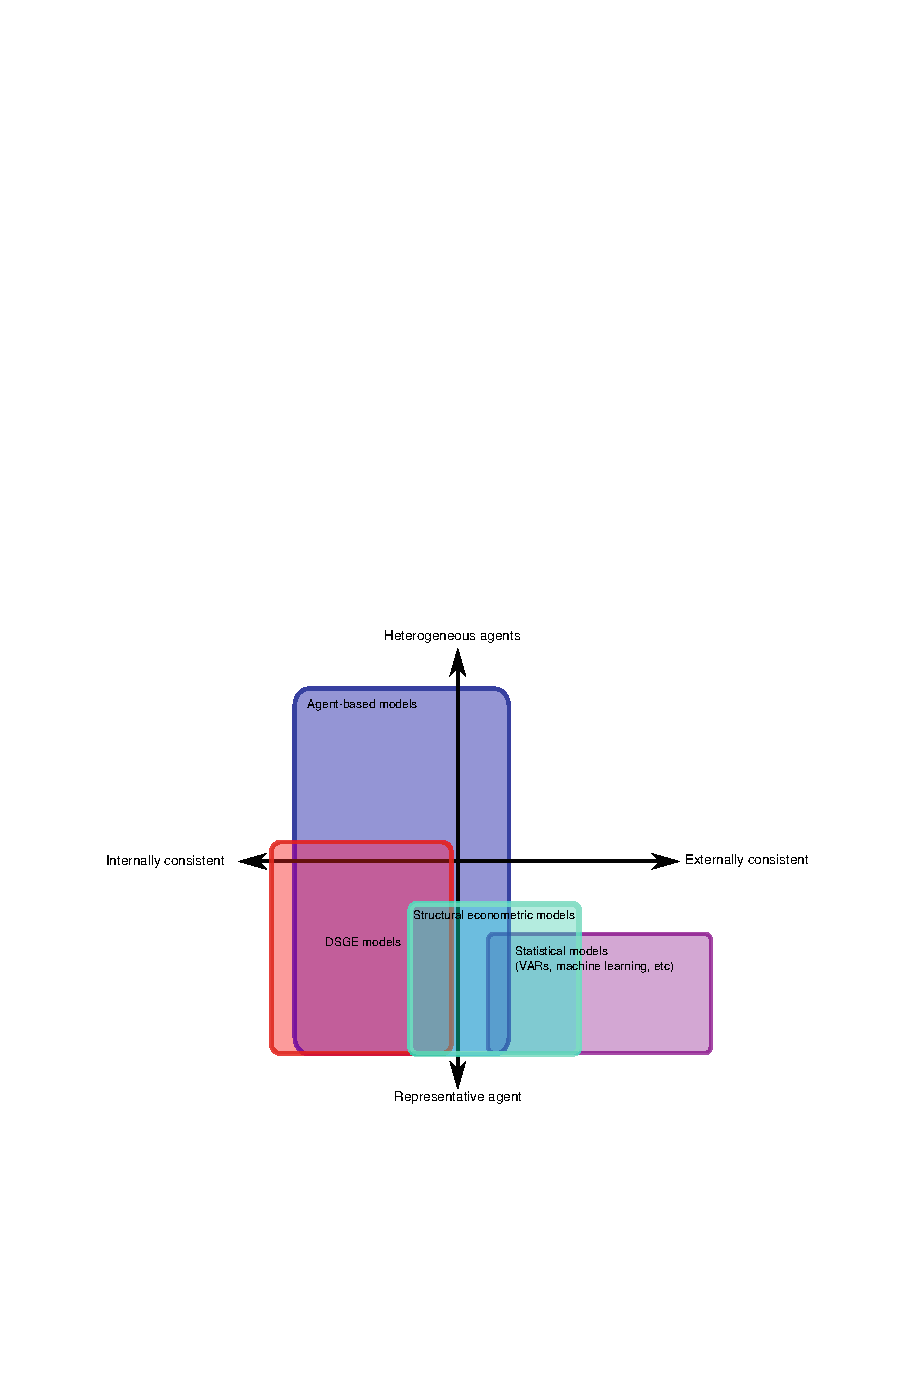
\includegraphics[width=0.8\linewidth]{ABMinEconomicsModelling.pdf}
    \caption{Macroeconomic modelling landscape}
    \label{fig:macroeconomicModellingLandscape}
\end{figure}

Moreover, they dive deeper into how ABMs compare to other models and what are the characteristics of Agent-Based Models. ABMs, encompass more behaviors and agents, making them bespoke and often criticized as \textit{black boxes}. In addition, ABMs are typically solved numerically at the agent level, contrasting with the analytical aggregation and linearization often employed in DSGE models. ABMs rely on numerical convergence, which might not perfectly match analytical solutions, but the error is often smaller than the error from inaccurate problem posing in macroeconomics. The real power of Agent-Based Models is the ability to generate multiple realizations of the world, allowing for experiments with different distributions and treatments, similar to real-world experiments.

Having in mind the characteristics of ABM, they are well suited for situations where agent interactions, heuristics, agent heterogeneity, agent-level policy implications, abundant granular data, and analytical limitations are crucial. They can be used to simulate non-clearing markets, capture emergent properties in financial networks, and model counter-intuitive macro-level behaviors arising from agent-level interactions.


One particular Agent-Based Model, that is worth mentioning as an example, was firstly proposed in 1994~\cite{yasutomiEmergenceCollapseMoney1995} and revisited in 2003~\cite{yasotumiItinerancyOfMoney2003} by Yasotumi. As R. Gębarowski et al. state in~\cite{gebarowskiAgentBasedModellingCommodity2016}, Yasutomi’s agent-based model of a commodity market could be perceived as a toy model rather than a fully fledged agent-based computational economics approach. Nonetheless, it proved to be quite useful for exposing some universal features of the complex systems in general, and economics markets in particular. Application of Yasutomi’s approach to modelling the commodity market allowed to reproduce some real market behaviour with statistical signatures of the money emergence phenomena as well as provided some evidence of the competition of commodities for a dominant status of the so-called commodity-based money.


% %%%%%%%%%%%%%%%%%%%%%%%%%%%%%%%%%%%%%%%%%%%%%%%%%%%%%%%%%%%%%%%%%%%%%%%%%%%%%%%
\section{\SectionTitleProblemSolution}
\label{sec:solution}

% % the following content of the section should be removed from the final version of the report.

\emph{Research problem formulation. Proposal of the solution: detailed description of the algorithms/system/framework.}

The exact simulation model proposed in this paper is \textbf{Wealth Distribution Simulation} - an Agent-Based Socioeconomic Modelling.

\subsection{Introduction}

This project implements an agent-based simulation model to explore the dynamics of wealth distribution in a simplified society. The primary motivation for developing this simulation model is to explore how individual-level socio-economic characteristics and spatial interactions can affect the spread and concentration of wealth in a society over time.

This simulation focuses on a simplified socio-economic environment in which individuals (agents) possess attributes such as wealth, income, education, age, and spatial location. These agents interact, move, age, learn, reproduce, and die – all of which affect the evolution of the simulated society. The model captures mechanisms such as income growth through education and experience, inheritance through intergenerational wealth transfer, and localized economic exchange influenced by individual traits.

\subsection{Agent Society}

The simulation is centered around a population of agents, each representing an individual with a certain amount of wealth. These agents engage in random transactions that redistribute wealth among themselves. To introduce more realistic and localized interaction patterns, agents live and interact with each other in a two-dimensional space. In this configuration, each agent occupies a position on a bounded continuous Cartesian coordinate system. The spatial embedding enables interactions to be conditioned on physical proximity instead of for example randomly chosen pairs of individuals.

Initially, each agent is assigned a random position (x, y) within a bounded spatial domain. During each simulation iteration, agents perform a random movement. Specifically, each agent selects a random direction $\theta \in [0, 2\pi)$ and a random distance $\delta \in [0, \delta_{max}]$, and updates its position according to equations:

\begin{equation}
    x' = x + \delta cos(\theta)
\end{equation}
\begin{equation}
    y' = y + \delta sin(\theta)
\end{equation}

After all agents have moved, pairwise interactions are evaluated based on Euclidean distance. If two agents are within a predefined interaction radius $r$ (i.e., $||\text{agent}_i - \text{agent}_l|| < r$), they are considered to have “encountered” each other, and a wealth exchange transaction is triggered.

By embedding agents in space and enabling movement-driven encounters, the simulation gains a more realistic and complex dynamic structure.

\subsection{Agent as individual}
\label{sec:agent-as-individual}

In this simulation, each agent represents an individual in a simplified society. Agents are designed with several characteristics that influence how they interact with others and how their economic situation evolves over time. These characteristics include spatial position, wealth, income, education, and age.

\begin{itemize}

    \item \textbf{Spatial position} \\
        Each agent has a position in a two-dimensional space, represented by (x, y) coordinates. This space allows agents to move around and only interact with nearby agents. In each simulation round, an agent randomly chooses a direction and a distance (up to a fixed limit) and moves accordingly. If two agents end up close enough to each other, they may perform a transaction.
        
    \item \textbf{Wealth} \\
        An agent’s wealth represents the total amount of resources or money they currently have. It changes over time due to income, transactions with other agents, taxation, and possibly redistribution. Transactions only happen between agents that are physically close in the simulation space.
        
    \item \textbf{Income} \\
        Agents earn income every round, which depends on their education level and age. The more educated or older (up to a point) an agent is, the higher their income tends to be. This is modelled as a simple linear relationship:
        \begin{equation}
             wealth_{t + 1} = wealth_{t} + (\alpha * education + \beta * age)
        \end{equation}
        where $\alpha$ and $\beta$ are constants that determine how strongly education and age influence income.

    \item \textbf{Consumption} \\
        In every iteration, agents face regular expenses that reduce their wealth before any transactions or income are applied. Consumption is modelled in two parts: (1: $base\_cons$) fixed amount spent on basic needs to cover essential costs like housing, food, utilities and transport and (2: $add\_cons$) "personal" expenses that can be understood as hobbies, leisure or unexpected purchases which is expressed as a customizable fraction of each agent's wealth. This captures the variability in individuals’ spending habits and introduces extra fluctuations in wealth trajectories. The whole consumption is represented by the following equation:

        \begin{equation}
            wealth_{t + 1} = wealth_{t} - max(base\_cons + add\_cons * (wealth_{t} - base\_cons), 0)
        \end{equation}
        
    \item \textbf{Education} \\
        Education is represented as a numeric level that can increase over time. Agents have a chance to improve their education in each round, simulating learning or training. However, education is capped at a maximum level to keep it realistic. Education level improvements in each iteration are controlled by a following equation:

        \begin{equation}
            edu\_lvl_{t + 1} = min(edu\_lvl_{t} + (lr * (1 - edu\_lvl_{t} / max\_edu\_lvl)), max\_edu\_lvl)
        \end{equation}

        where $lr$ is a randomly generated learning rate from range $[min\_lr, max\_lr)$, which is adjustable in simulation configuration.
        
    \item \textbf{Age and death} \\
        Every agent has an age that increases with each round. As agents get older, their probability of dying also increases based on the sigmoid probability function described below:

        \begin{equation}
            death\_prob = \frac{1}{( 1 + e^{-1 * steepness * (age_{t} - mid\_age)} )}
        \end{equation}

        where $mid\_age$ is the age in years when the probability of death should reach $50\%$ and $steepness$ is controlling how sharply the death probability increases with age. This is a basic way to simulate population turnover.
        
\end{itemize}

By combining these features, the agents can simulate a variety of real-world social and economic behaviors. The model can capture how wealth and opportunity accumulate or spread over time, how mobility and proximity affect interaction, and how education and age shape economic outcomes. This richer agent design lays the groundwork for studying inequality, social mobility, and the effects of policy decisions in a more dynamic and realistic way.

\subsection{Transactions}
\label{sec:transactions}

Economic transactions occur when two agents encounter each other in space – that is, when they move close enough during a simulation round. These interactions simulate the kind of local trade or exchange that happens in real-world social and economic settings.

The process of transcation is as follows:

\begin{enumerate}
    \item \textbf{Detecting an Encounter} \\
        After all agents have moved during a given round, the simulation checks for pairs of agents that are within a specified interaction radius. If two agents are close enough, a transaction is triggered between them.
    \item \textbf{Determining the Transaction Amount} \\
        The amount of money that will be transferred is randomly determined as a small percentage of the poorer agent’s current wealth. This ensures that interactions are bounded by what the agents can afford, and keeps the model realistic by preventing extreme losses or gains from a single transaction.
    \item \textbf{Choosing the Winner (Biased Coin Flip)} \\
        The direction of the transaction – that is, who gives and who receives – is decided using a biased coin flip. The bias is based on each agent’s education and age, which are treated as proxies for skill, experience, or negotiation power. The more educated and older an agent is, the higher their chances of “winning” the transaction and receiving the money. This models the idea that people with more knowledge or life experience may be better at securing favorable outcomes in economic interactions.
    \item \textbf{Applying Taxes} \\
        After the transaction amount is transferred to the winning agent, a fixed percentage (e.g., 5\%) of that amount is deducted as a tax. This simulates basic government taxation or friction in the economy. The taxed amount is collected for the analysis.
\end{enumerate}

\subsection{Agent Lifecycle}

The simulation begins with a population of agents, each initialized with randomized but realistic values for wealth, education, income, and age. These values are sampled from predefined distributions to ensure diversity in the population’s socioeconomic status. From that point forward, each agent evolves over time according to a defined life cycle that includes aging, income growth, potential death, and reproduction.

\textbf{Aging and mortability} \\
At the end of each simulation round, every agent’s age is incremented by one. As agents get older, their probability of dying increases. This probability is modeled using a simple age-dependent mortality function (for example, a linearly increasing or sigmoidal curve), so that older agents are more likely to exit the simulation. This mechanism introduces generational turnover and ensures that the population evolves over time.

\textbf{Death and Reproduction} \\
When an agent dies, the simulation immediately initiates a reproduction event to maintain a stable population size. Two other agents, selected randomly from those in the reproductive age range, are chosen to be the parents of a new agent. These parents remain in the simulation, but their wealth is partially transferred to the offspring. The child agent starts with minimal levels of education and baseline income.

To determine the child’s starting wealth, a weighted inheritance mechanism is used. The total combined wealth of both parents is multiplied by a random fraction, constrained such that the child receives at least 20\% of each parent’s wealth.

This reflects the idea that offspring are born into a socioeconomic situation influenced by their parents’ status, while still allowing variability and randomness to simulate unequal inheritance or chance-based opportunity.

\textbf{Education and Income Growth} \\
Since new agents start at the lowest levels of education and income, their economic capabilities must grow over time. During each round, an agent has a chance to increase their education level, up to a fixed maximum. As education and age increase, so does the agent’s income, following a linear income model. This setup allows agents to “climb the ladder” economically over time, contributing to long-term emergent behavior in the simulation such as wealth stratification.

\subsection{Metrics}

To assess the behavior of the simulation, several key metrics are tracked and analyzed over time. These metrics help evaluate both the internal state of the agent population and the macro-level outcomes that emerge from agent interactions as the society evolves.

At each simulation step, the \textbf{distribution of wealth} among agents is recorded. This includes basic statistics such as mean and median, minimum and maximum, standard deviation and variance. These metrics give an overview of how wealth is concentrated or dispersed in the population over time.

\textbf{The Gini coefficient} is a standard measure of inequality. A Gini coefficient of 0 indicates perfect equality (everyone has the same wealth), while a value close to 1 indicates extreme inequality. Tracking this value over time reveals whether the system trends toward fairness or concentration of wealth.

Moreover, the number of \textbf{transactions}, average transaction amount, and total wealth exchanged are recorded. This helps understand the scale and frequency of economic interactions.

The simulation tracks the average \textbf{education level} of agents, as well as its distribution. This can show whether access to education improves over generations and how it correlates with economic outcomes.

% %%%%%%%%%%%%%%%%%%%%%%%%%%%%%%%%%%%%%%%%%%%%%%%%%%%%%%%%%%%%%%%%%%%%%%%%%%%%%%%
% \subsection{Equations}
% \label{sec:equations}

% Exemplary equation with reference to literature~\cite{author2021title}:

% \begin{equation}
% \Omega = \sum_{i=1}^n \gamma_i
% \label{eq:sum}
% \end{equation}

% Exemplary reference to Equation~\eqref{eq:sum}.

% Exemplary, unnumbered equation placed within the text: $\lambda = \sum_{i=1}^n \delta_i$.

% %%%%%%%%%%%%%%%%%%%%%%%%%%%%%%%%%%%%%%%%%%%%%%%%%%%%%%%%%%%%%%%%%%%%%%%%%%%%%%%
% \subsection{Algorithms}
% \label{sec:algorithms}

% Listing~\ref{lst:maximum} shows an exemplary fragment of source code.

% \begin{lstlisting}[language=Python,float=!htbp,caption={Exemplary fragment of source code (source:
%   \cite{author2021title})},label=lst:maximum]
% # The maximum of two numbers

% def maximum(x, y):

%     if x >= y:
%         return x
%     else:
%         return y

% x = 2
% y = 6
% print(maximum(x, y),"is the largest of the numbers ", x, " and ", y)

% \end{lstlisting}

% Algorithm~\ref{alg:pseudo-code} shows an exemplary pseudo-code presented in~\cite{fiorio2017algorithm2e}.

% \begin{algorithm}[!htbp]
% \SetKwData{Left}{left}\SetKwData{This}{this}\SetKwData{Up}{up}
% \SetKwFunction{Union}{Union}\SetKwFunction{FindCompress}{FindCompress}
% \SetKwInOut{Input}{input}\SetKwInOut{Output}{output}
% \Input{A bitmap $Im$ of size $w\times l$}
% \Output{A partition of the bitmap}
% \BlankLine
% \emph{special treatment of the first line}\;
% \For{$i\leftarrow 2$ \KwTo $l$}{
% \emph{special treatment of the first element of line $i$}\;
% \For{$j\leftarrow 2$ \KwTo $w$}{\label{forins}
% \Left$\leftarrow$ \FindCompress{$Im[i,j-1]$}\;
% \Up$\leftarrow$ \FindCompress{$Im[i-1,]$}\;
% \This$\leftarrow$ \FindCompress{$Im[i,j]$}\;
% \If(\tcp*[h]{O(\Left,\This)==1}){\Left compatible with \This}{\label{lt}
% \lIf{\Left $<$ \This}{\Union{\Left,\This}}
% \lElse{\Union{\This,\Left}}
% }
% \If(\tcp*[f]{O(\Up,\This)==1}){\Up compatible with \This}{\label{ut}
% \lIf{\Up $<$ \This}{\Union{\Up,\This}}
% \tcp{\This is put under \Up to keep tree as flat as possible}\label{cmt}
% \lElse{\Union{\This,\Up}}\tcp*[h]{\This linked to \Up}\label{lelse}
% }
% }
% \lForEach{element $e$ of the line $i$}{\FindCompress{p}}
% }
%   \caption[Exemplary algorithm]{Exemplary algorithm (source: \cite{fiorio2017algorithm2e}).}
%   \label{alg:pseudo-code}
% \end{algorithm}

% %%%%%%%%%%%%%%%%%%%%%%%%%%%%%%%%%%%%%%%%%%%%%%%%%%%%%%%%%%%%%%%%%%%%%%%%%%%%%%%
\section{\SectionTitleExperiments}
\label{sec:experiments}

% % the following content of the section should be removed from the final version of the report.

\emph{Experimental research results with detailed analyses and comments.}

\subsection{Available simulation parameters}

    The simulation model has multiple customizable parameters that can be provided before the simulation starts in order to tweak the process and behaviour of the simulation. These parameters are:

    \begin{itemize}
        \item number of iterations
        \item number of agents
        \item size of the simulation space (length and width in points)
        \item interaction radius – size of the surrounding space around each agent in which the interaction can happen
        \item maximal agent's movement in one iteration (in points)
        \item agents' age and death probability parameters:
            \begin{itemize}
                \item mean initial age of agents during the initialization
                \item standard deviation of agents' age during the initialization
                \item maximal initial age of agents during the initialization
                \item age of agents' in which the death probability is $50\%$
                \item steepness of the sigmoid function responsible for modelling death probability over age
            \end{itemize}
        \item education parameters:
            \begin{itemize}
                \item minimal and maximal education levels of adult agents during initialization
                \item elementary education level
                \item maximal education level
                \item children education level jitter
                \item minimal and maximal learning rate for increasing the agents' education level over time
            \end{itemize}
        \item income and consumption parameters:
            \begin{itemize}
                \item weight of the education level parameter (denoted in Section \ref{sec:agent-as-individual} as $\alpha$)
                \item weight of the age parameter (denoted in Section \ref{sec:agent-as-individual} as $\beta$)
                \item the amount of agent's wealth spent on base consumption needs
                \item the percentage of agent's wealth spent on additional consumption needs
            \end{itemize}
        \item transaction parameters:
            \begin{itemize}
                \item transaction probability
                \item education level weight – a parameter for determining the winner of the transaction based on Section \ref{sec:transactions}
                \item age weight – a parameter for determining the winner of the transaction based on Section \ref{sec:transactions}
                \item tax rate – what percentage of the transaction amount is considered a tax
                \item amount rate – what percentage of poorer agent's wealth is considered as a transaction amount
            \end{itemize}
        \item wealth parameters:
            \begin{itemize}
                \item minimal and maximal initial wealth of each agent during the initialization
                \item minimal and maximal inheritance rates at the birth of new agents 
            \end{itemize}
    \end{itemize}

\subsection{Visualizations of performed metrics}

    For each set of parameters (also called configuration), the following metrics are calculated and visualized in the form of line plots:

    \begin{itemize}
        \item total transactions' amount over iterations
        \item average transaction amount over iterations
        \item total number of transactions (count) over iterations
        \item Gini coefficient of population's wealth over iterations
        \item population's wealth percentiles over iterations
        \item total population's wealth over iterations
        \item number of adult agents over iterations
        \item death probability curve
        \item mean education level over iterations
        \item education level percentiles over iterations
    \end{itemize}

\subsection{Baseline configuration \& its visualizations}

    As a baseline, the following set of parameters is used:

    \captionof{listing}{Baseline Configuration (\textit{Configuration 0})}
    \begin{minted}{json}
{
  "num_iterations": 30000,
  "num_agents": 1000,
  "length": 1000,
  "width": 1000,
  "interaction_radius": 50.0,
  "max_movement": 15.0,
  "age_and_death": {
    "mean_age": 30.0,
    "stddev_age": 10.0,
    "mid_age": 80.0,
    "max_start_age": 90.0,
    "steepness": 0.02
  },
  "education": {
    "initial_adult_min": 4.0,
    "initial_adult_max": 10.0,
    "elemental_education_threshold": 4.0,
    "children_education_jitter": 2.0,
    "learning_rate_min": 0.005,
    "learning_rate_max": 0.05,
    "max": 10.0
  },
  "income_and_consumption": {
    "income_age_parameter": 0.05,
    "income_education_parameter": 2.0,
    "base_consumption": 10.0,
    "aditional_consumption_rate": 0.2
  },
  "transaction": {
    "transaction_probability": 0.3,
    "education_parameter": 1.0,
    "age_parameter": 0.001,
    "tax_rate": 0.05,
    "amount_rate": 0.05
  },
  "wealth": {
    "min_initial_wealth": 10.0,
    "max_initial_wealth": 100.0,
    "min_inheritance_at_birth_rate": 0.1,
    "max_inheritance_at_birth_rate": 0.3
  }
}
    \end{minted}

    The computed metrics in the form of line plots:

    \begin{figure}[H]
        \centering
        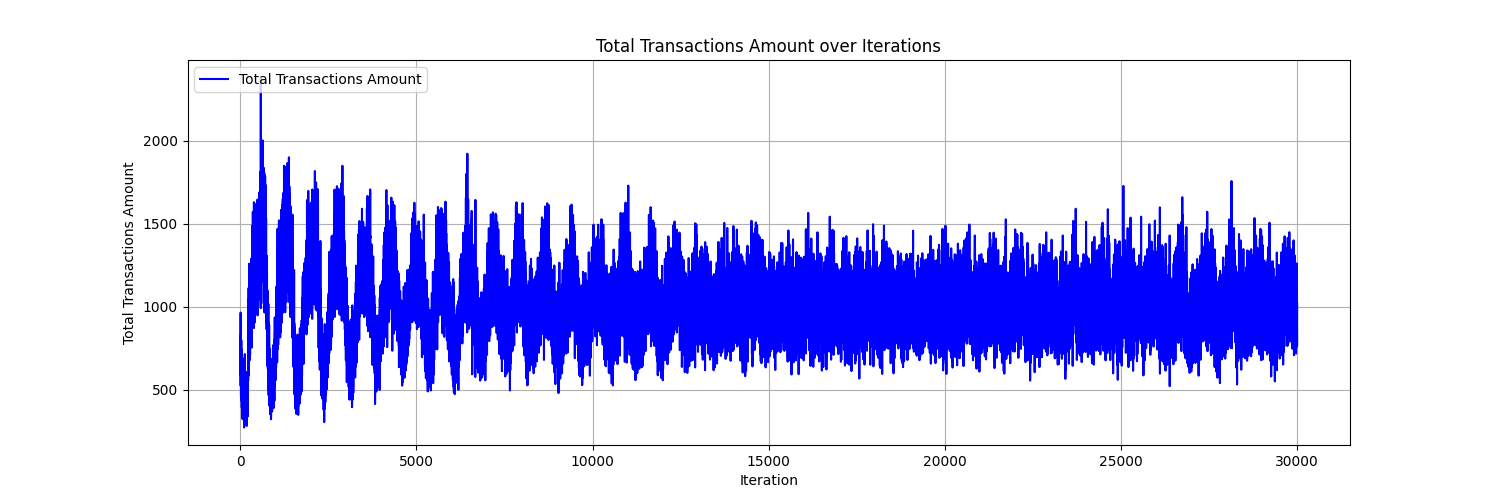
\includegraphics[width=0.8\linewidth]{metrics_config0/metrics_config0_total_transactions_amount.png}
        \caption{Configuration 0: Total transactions' amount over iterations}
        \label{fig:c0-total_transactions_amount}
    \end{figure}

    \begin{figure}[H]
        \centering
        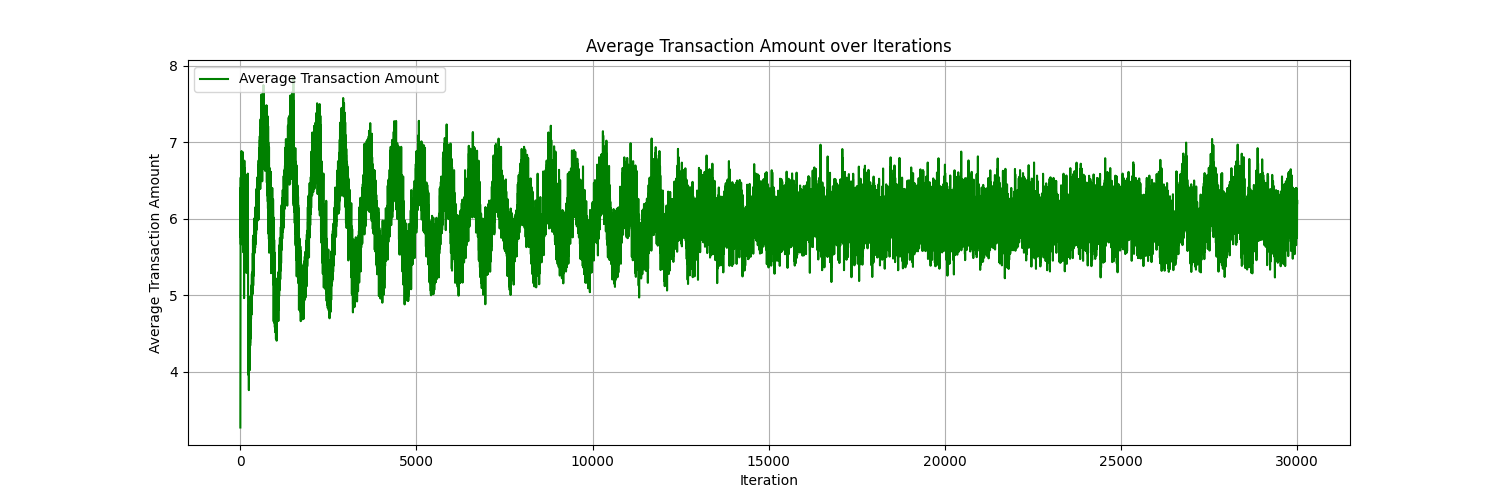
\includegraphics[width=0.8\linewidth]{metrics_config0/metrics_config0_average_transaction_amount.png}
        \caption{Configuration 0: Average transaction amount over iterations}
        \label{fig:c0-average_transaction_amount}
    \end{figure}

    \begin{figure}[H]
        \centering
        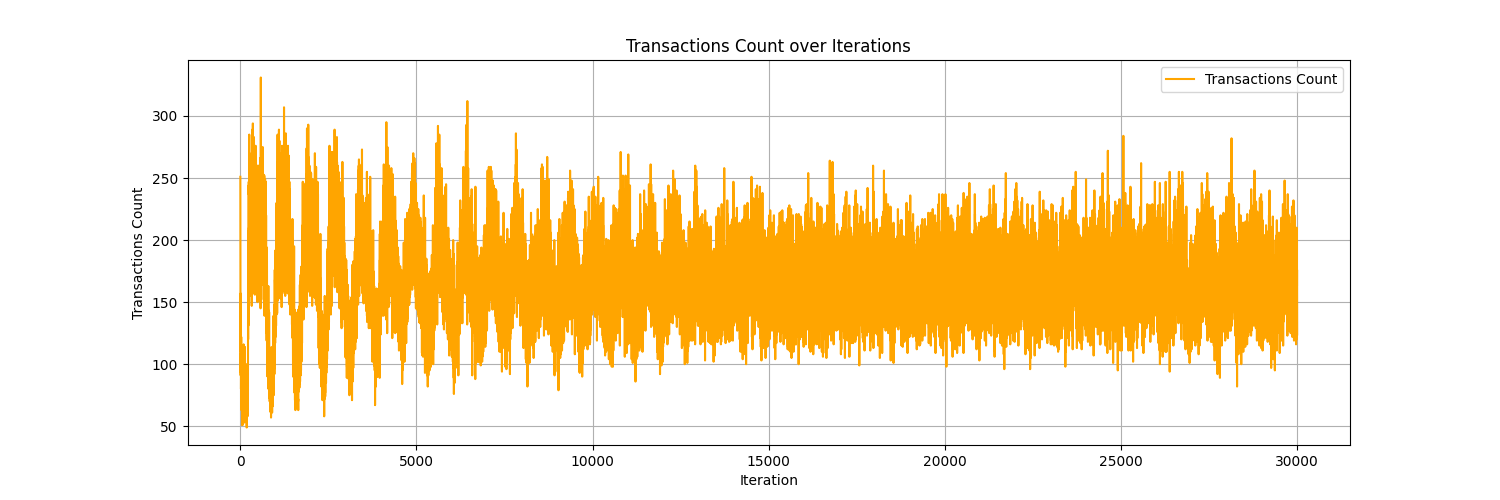
\includegraphics[width=0.8\linewidth]{metrics_config0/metrics_config0_total_transactions_count.png}
        \caption{Configuration 0: Total number of transactions (count) over iterations}
        \label{fig:c0-total_transactions_count}
    \end{figure}

    \begin{figure}[H]
        \centering
        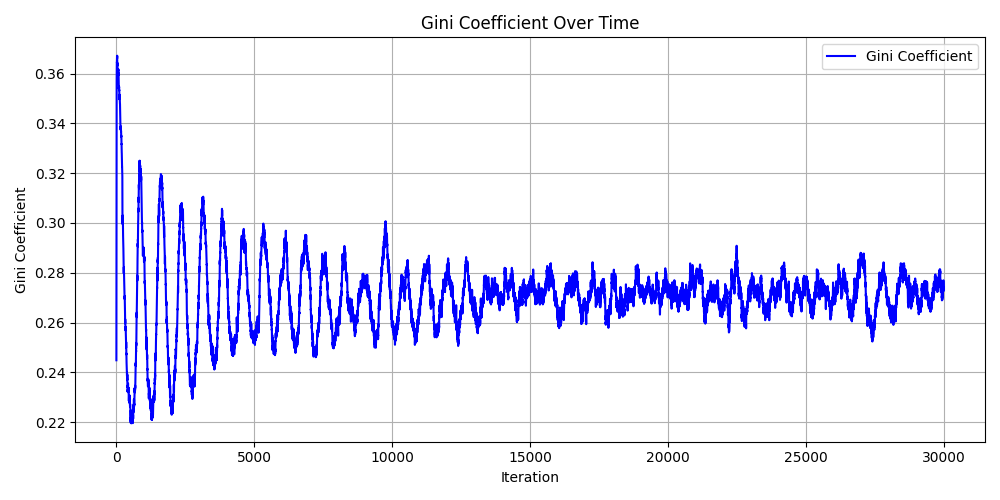
\includegraphics[width=0.8\linewidth]{metrics_config0/metrics_config0_gini_coefficient.png}
        \caption{Configuration 0: Gini coefficient of population's wealth over iterations}
        \label{fig:c0-gini_coefficient}
    \end{figure}

    \begin{figure}[H]
        \centering
        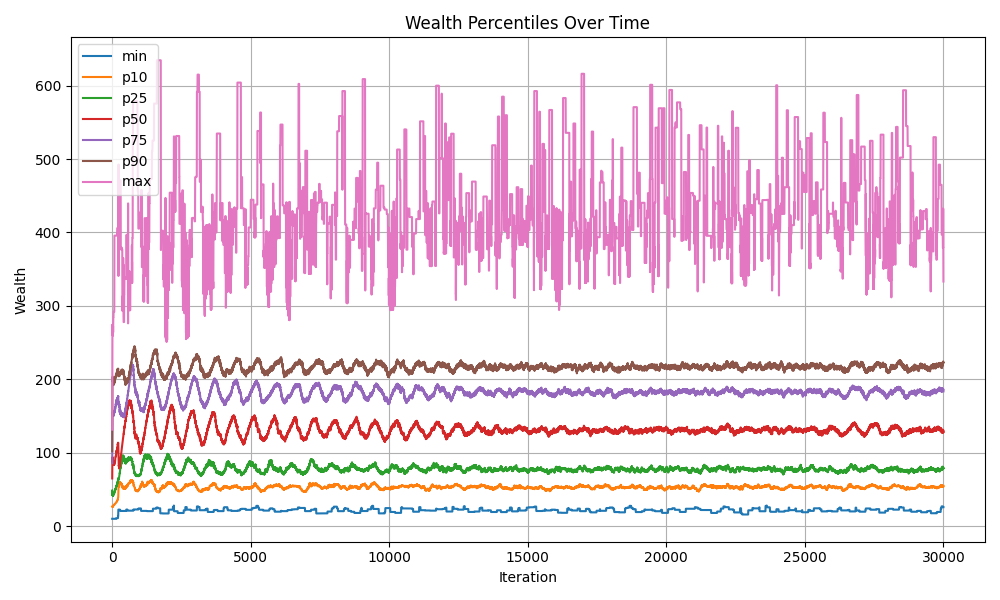
\includegraphics[width=0.8\linewidth]{metrics_config0/metrics_config0_wealth_perc_time.png}
        \caption{Configuration 0: Population's wealth percentiles over iterations}
        \label{fig:c0-wealth_perc_time}
    \end{figure}

    \begin{figure}[H]
        \centering
        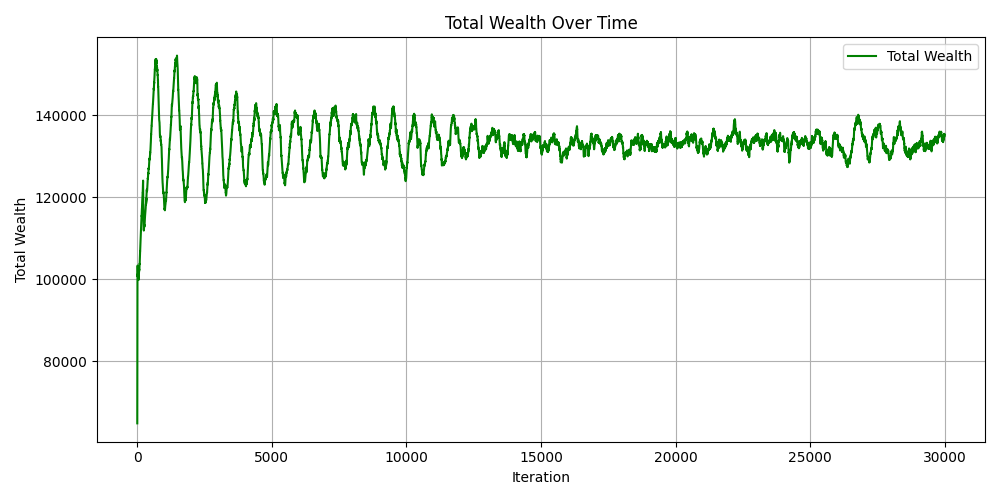
\includegraphics[width=0.8\linewidth]{metrics_config0/metrics_config0_total_wealth.png}
        \caption{Configuration 0: Total population's wealth over iterations}
        \label{fig:c0-total_wealth}
    \end{figure}

    \begin{figure}[H]
        \centering
        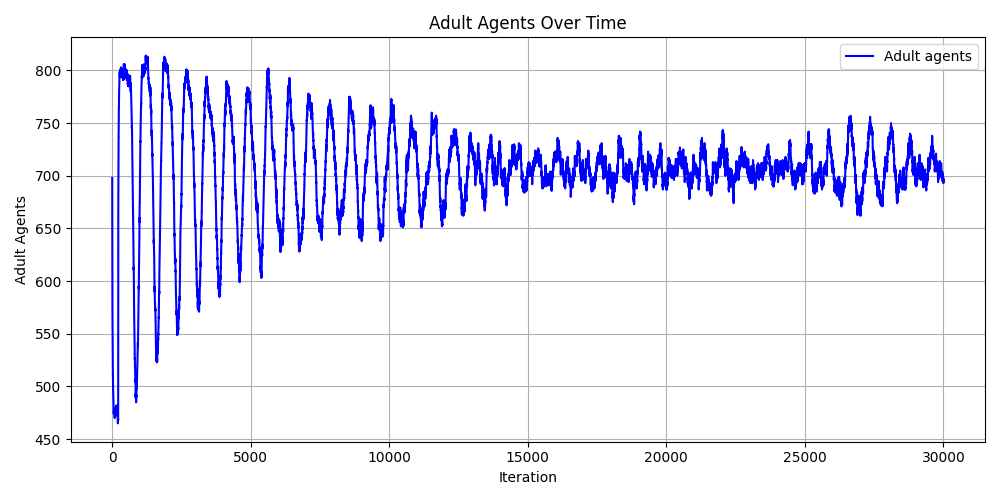
\includegraphics[width=0.8\linewidth]{metrics_config0/metrics_config0_adult_agents.png}
        \caption{Configuration 0: Number of adult agents over iterations}
        \label{fig:c0-adult_agents}
    \end{figure}

    \begin{figure}[H]
        \centering
        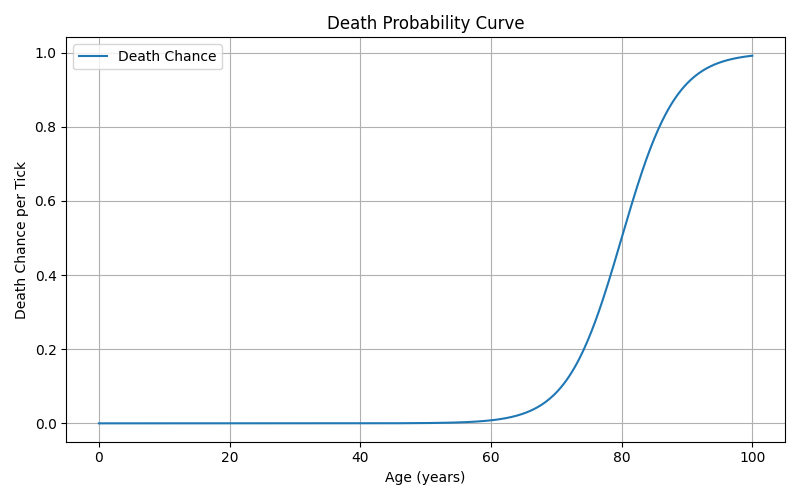
\includegraphics[width=0.8\linewidth]{metrics_config0/metrics_config0_death_probability_curve.png}
        \caption{Configuration 0: Death probability curve}
        \label{fig:c0-death_probability_curve}
    \end{figure}

    \begin{figure}[H]
        \centering
        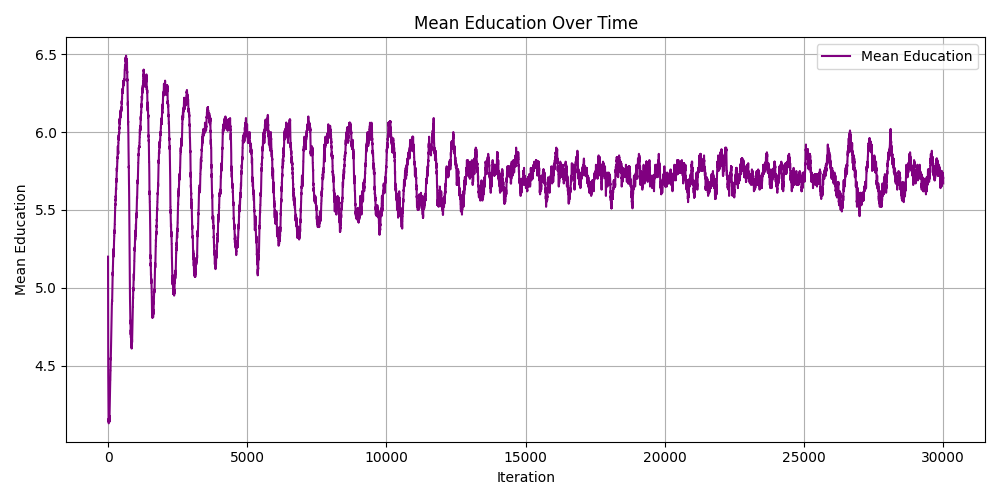
\includegraphics[width=0.8\linewidth]{metrics_config0/metrics_config0_mean_education.png}
        \caption{Configuration 0: Mean education level over iterations}
        \label{fig:c0-mean_education}
    \end{figure}

    \begin{figure}[H]
        \centering
        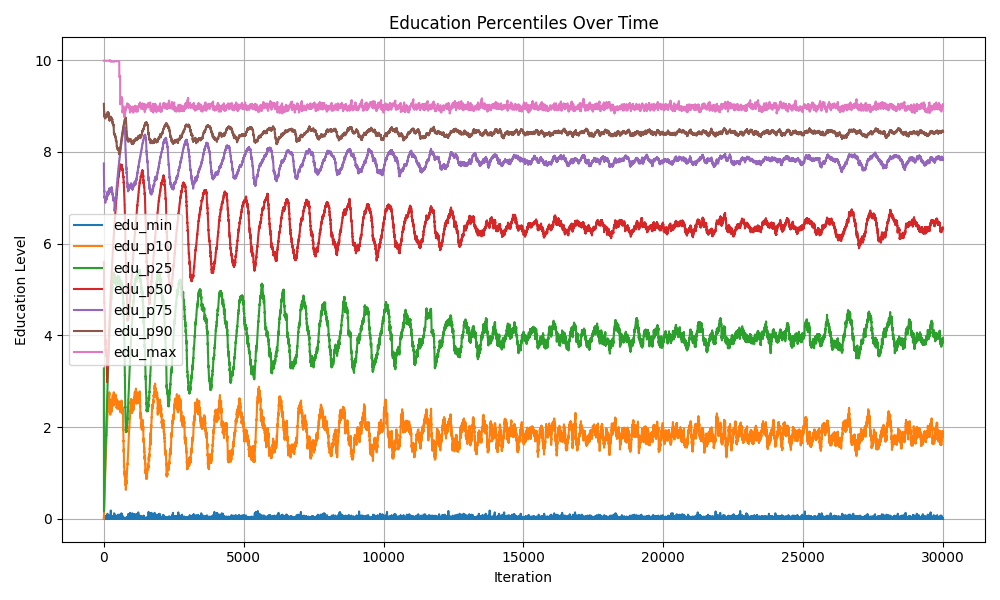
\includegraphics[width=0.8\linewidth]{metrics_config0/metrics_config0_education_perc_time.png}
        \caption{Configuration 0: Education level percentiles over iterations}
        \label{fig:c0-education_perc_time}
    \end{figure}

    On many charts (Fig. \ref{fig:c0-total_transactions_amount}, \ref{fig:c0-average_transaction_amount}, \ref{fig:c0-total_transactions_count}, \ref{fig:c0-wealth_perc_time}, \ref{fig:c0-gini_coefficient}, \ref{fig:c0-total_wealth}, \ref{fig:c0-adult_agents}, \ref{fig:c0-mean_education}, \ref{fig:c0-education_perc_time}), we can see that in the first 12 thousand iterations, the simulation needs to \textit{warm up} since there are higher oscillations in different metrics. Then, the simulation steadies and all metrics become more stable.

    The Gini coefficient plot (Fig. \ref{fig:c0-gini_coefficient}) shows that the selected set of parameters is stable between $0.26$ and $0.28$ which means the society is relatively equal.

    The death probability curve on Fig. \ref{fig:c0-death_probability_curve} provides insight about the probability of how long agents are supposed to live.

    \vspace{5mm} %5mm vertical space

    In the next configurations, we iteratively modified each subset of parameters and now we will show how these changes affect the simulation. In order to provide concise comparisons, we will focus only on those parts of metrics that represent differences between configurations. The baseline configuration will be called \textit{Configuration 0}.

\subsection{Configuration 1: Environment \& age and death parameters}

\begin{minipage}{0.48\textwidth}
\captionof{listing}{Configuration 0}
\begin{minted}[fontsize=\small]{json}
{
  // ...
  "length": 1000,
  "width": 1000,
  "interaction_radius": 50.0,
  "max_movement": 15.0,
  "age_and_death": {
    "mean_age": 30.0,
    "stddev_age": 10.0,
    "mid_age": 80.0,
    "max_start_age": 90.0,
    "steepness": 0.02
  },
  // ...
}
\end{minted}
\end{minipage}
\hfill
\begin{minipage}{0.48\textwidth}
\captionof{listing}{Configuration 1}
\begin{minted}[fontsize=\small]{json}
{
  // ...
  "length": 1500,
  "width": 1500,
  "interaction_radius": 75.0,
  "max_movement": 20.0,
  "age_and_death": {
    "mean_age": 35.0,
    "stddev_age": 15.0,
    "mid_age": 80.0,
    "max_start_age": 70.0,
    "steepness": 0.02
  },
  // ...
}
\end{minted}
\end{minipage}

    This configuration modifies the environment parameters such as the size of the simulation space, interaction radius, maximal movement, and age and death parameters subset.

    Performed changes make the simulation more stable from the beginning as it does not oscillate so much in the first couple of thousand iterations. The cause of this difference is based on tweaking the age and death parameters, especially the standard deviation of initial agents' age and the decrease in the maximal initial agents' age.

    This change can be shown on multiple metrics, but here we will use plots for transaction count and total wealth over iterations:

\begin{figure}[H]
\begin{center}
\subfigure{%
\label{fig:c0-total_transactions_count-2}
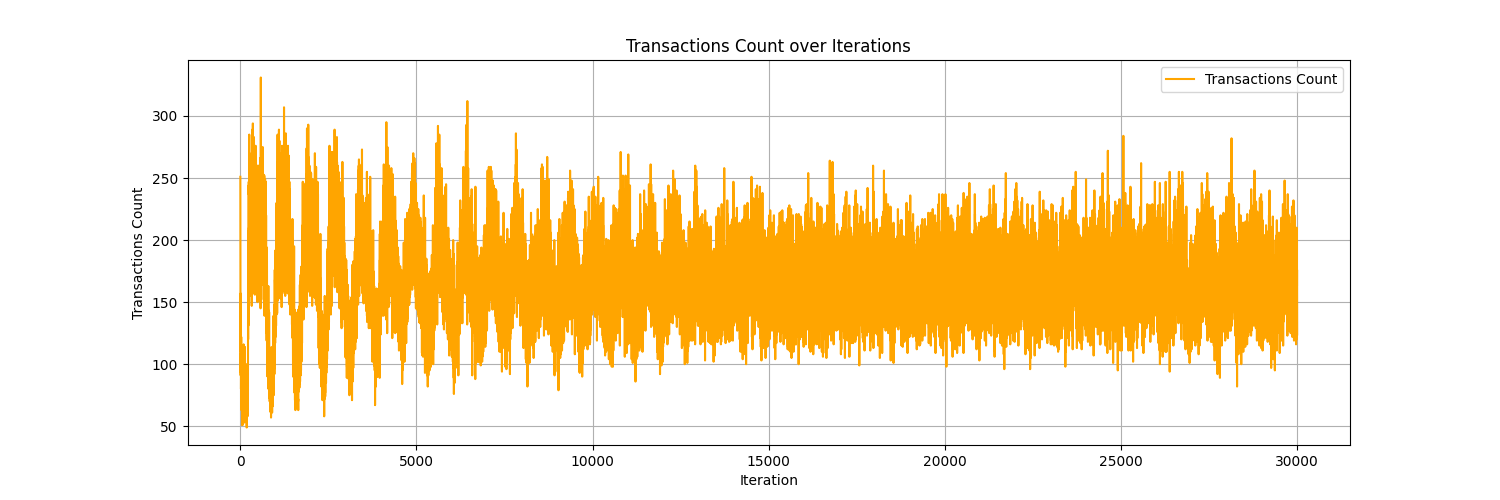
\includegraphics[width=0.48\textwidth]{metrics_config0/metrics_config0_total_transactions_count.png}}%
\subfigure{%
\label{fig:c0-total_transactions_amount}
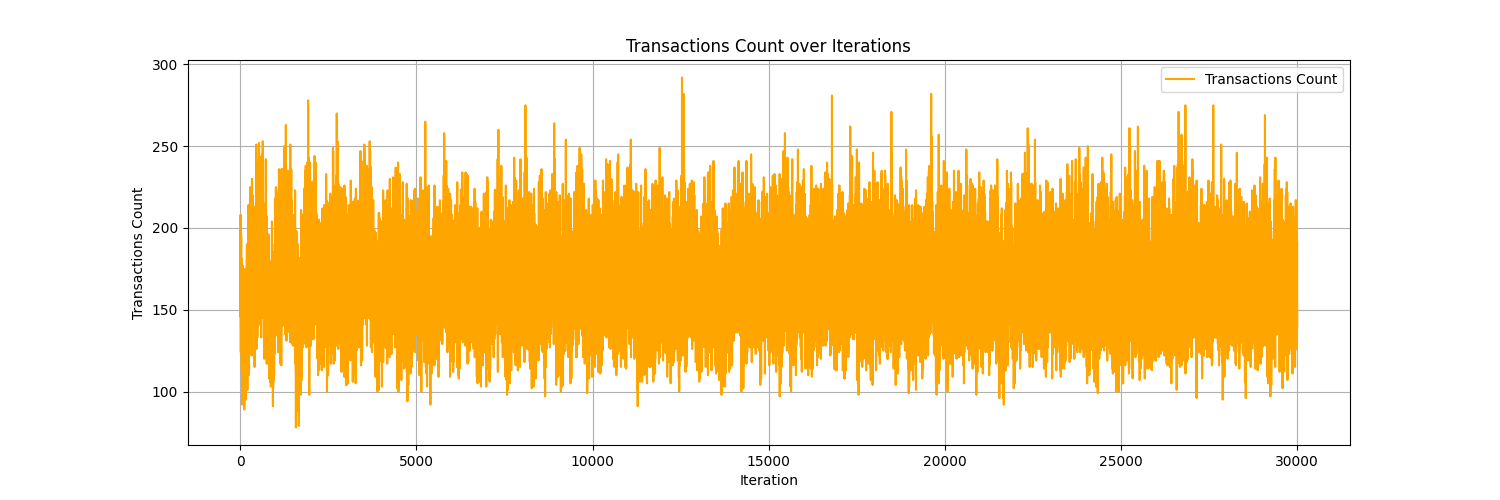
\includegraphics[width=0.48\textwidth]{metrics_config1/metrics_config1_total_transactions_count.png}}
\label{fig:c1-total_transactions_count}
\end{center}
\caption{The difference in transactions count over iterations between Configuration 0 (left) and Configuration 1 (right)}
\end{figure}

\begin{figure}[H]
\begin{center}
\subfigure{%
\label{fig:c0-total_wealth-2}
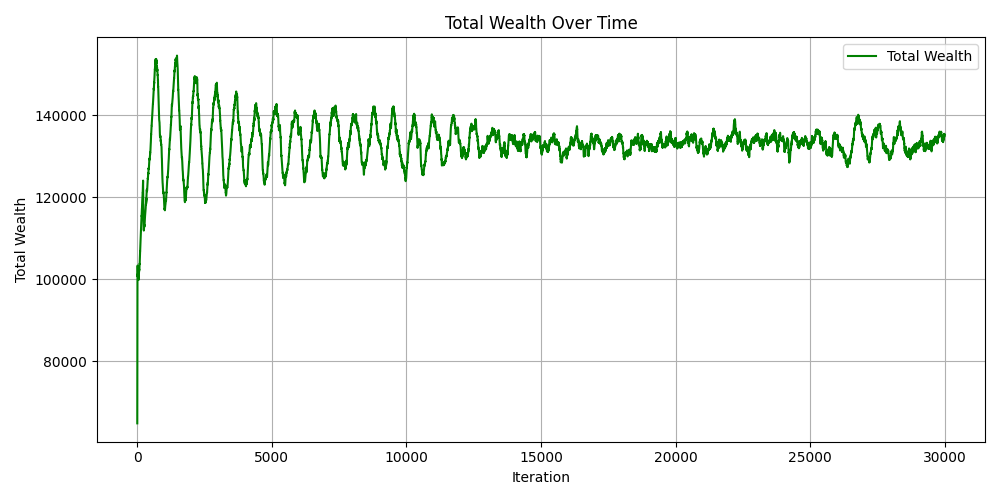
\includegraphics[width=0.48\textwidth]{metrics_config0/metrics_config0_total_wealth.png}}%
\subfigure{%
\label{fig:c0-total_transactions_amount}
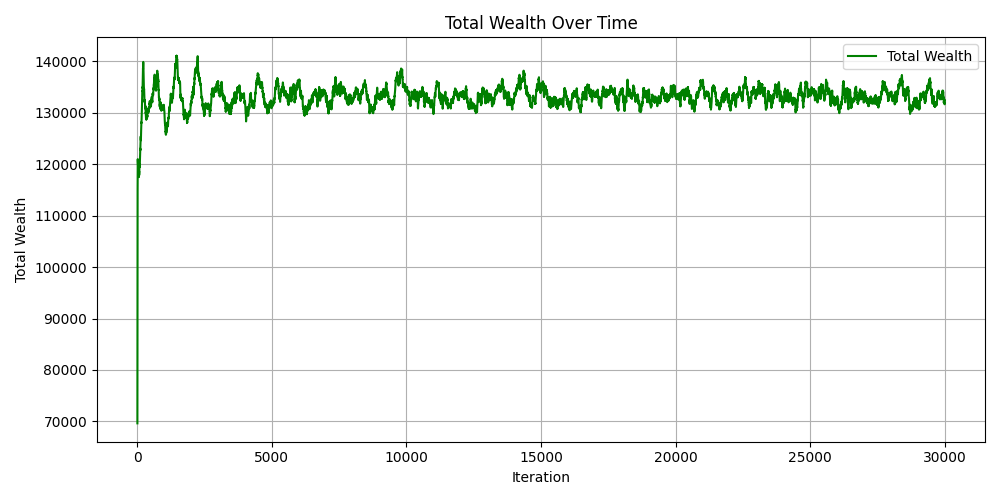
\includegraphics[width=0.48\textwidth]{metrics_config1/metrics_config1_total_wealth.png}}
\label{fig:c1-total_wealth}
\end{center}
\caption{The difference in total wealth over iterations between Configuration 0 (left) and Configuration 1 (right)}
\end{figure}


\subsection{Configuration 2: Education parameters}

\begin{minipage}{0.48\textwidth}
\captionof{listing}{Configuration 0 \& 1}
\begin{minted}[fontsize=\small]{json}
{
  // ...
  "education": {
    "initial_adult_min": 4.0,
    "initial_adult_max": 10.0,
    "elemental_education_threshold": 4.0,
    "children_education_jitter": 2.0,
    "learning_rate_min": 0.005,
    "learning_rate_max": 0.05,
    "max": 10.0
  },
  // ...
}
\end{minted}
\end{minipage}
\hfill
\begin{minipage}{0.48\textwidth}
\captionof{listing}{Configuration 2}
\begin{minted}[fontsize=\small]{json}
{
  // ...
  "education": {
    "initial_adult_min": 3.0,
    "initial_adult_max": 10.0,
    "elemental_education_threshold": 3.0,
    "children_education_jitter": 2.0,
    "learning_rate_min": 0.001,
    "learning_rate_max": 0.1,
    "max": 10.0
  },
  // ...
}
\end{minted}
\end{minipage}

    This configuration modifies the environment parameters associated with education. It widens the education level range, decreases the elementary education level, and broadens the learning rate range.

    These changes lead to a higher amount of money per transaction and simultaneously to a higher total amount of money in transactions per iteration. Moreover, the total wealth over iterations increases and the population's Gini coefficient decreases from range $ \sim [0.26, 0.28]$ to range $ \sim [0.24, 0.26]$, which makes the society more equal.

    However, most important difference is visible on plots related to the education: by increasing the maximal learning rate from $0.05$ to $0.1$, the mean education level increases and overall all education level percentiles also increase, as shown on Fig. \ref{fig:c2-mean_education} and \ref{fig:c2-education_perc_time}.

\begin{figure}[H]
\begin{center}
\subfigure{%
\label{fig:c1-mean_education}
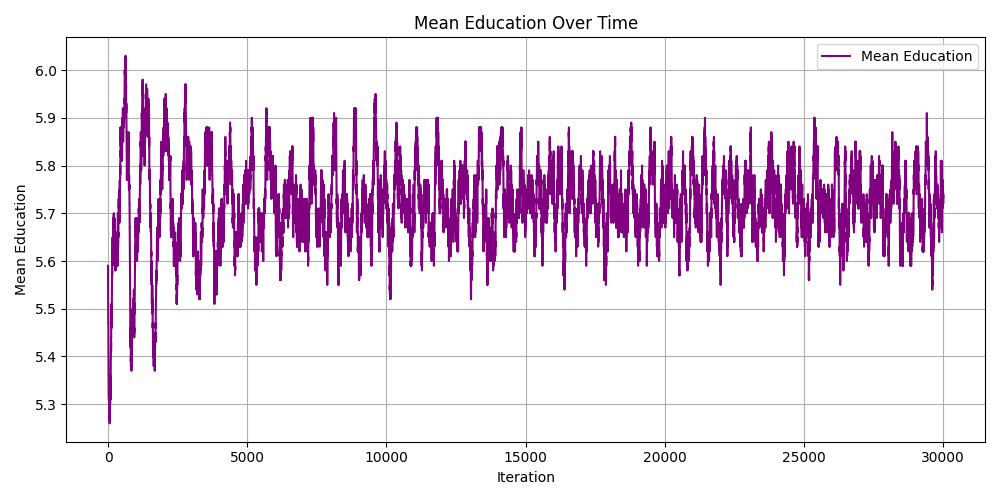
\includegraphics[width=0.48\textwidth]{metrics_config1/metrics_config1_mean_education.png}}%
\subfigure{%
\label{fig:c2-mean_education}
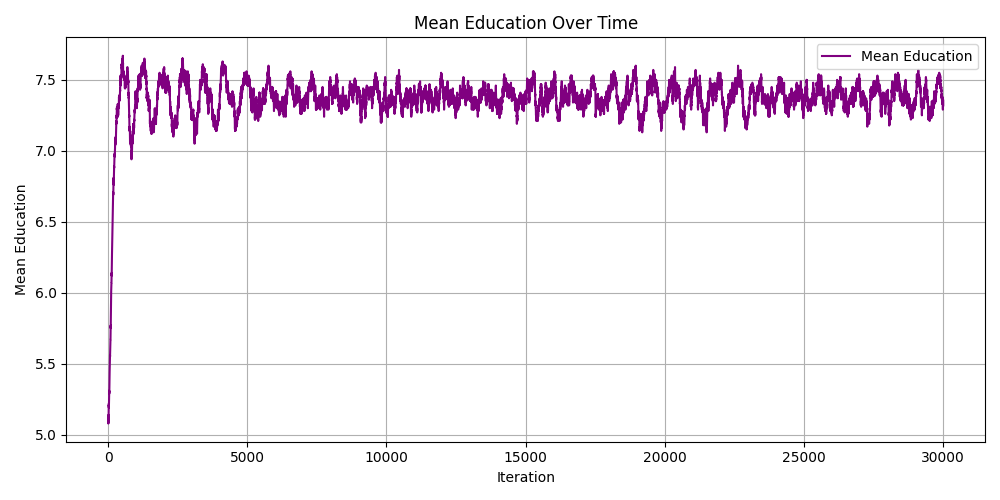
\includegraphics[width=0.48\textwidth]{metrics_config2/metrics_config2_mean_education.png}}
\end{center}
\caption{The difference in mean education level over iterations between Configuration 1 (left) and Configuration 2 (right)}
\end{figure}

\begin{figure}[H]
\begin{center}
\subfigure{%
\label{fig:c1-education_perc_time}
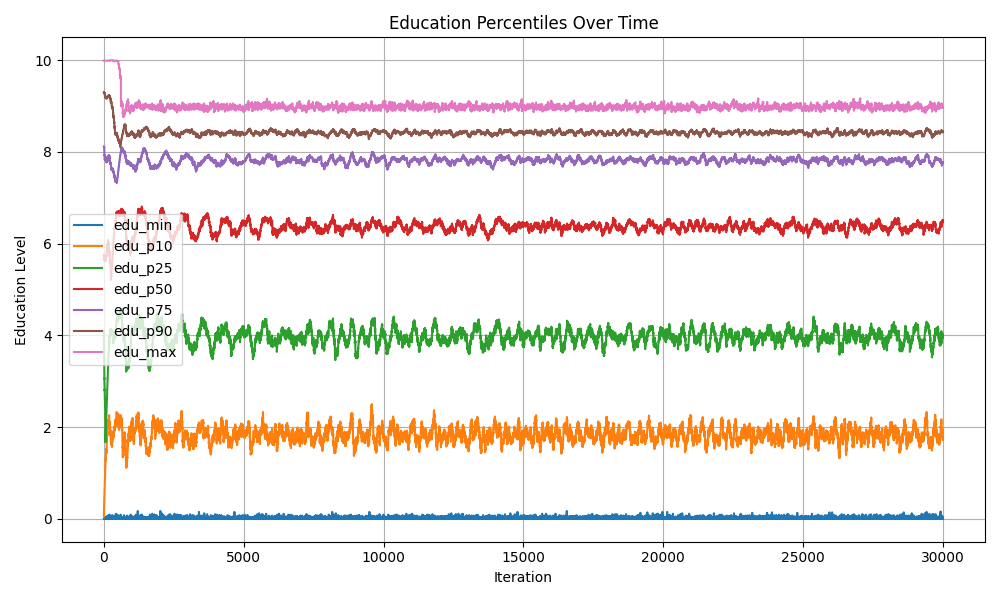
\includegraphics[width=0.48\textwidth]{metrics_config1/metrics_config1_education_perc_time.png}}%
\subfigure{%
\label{fig:c2-education_perc_time}
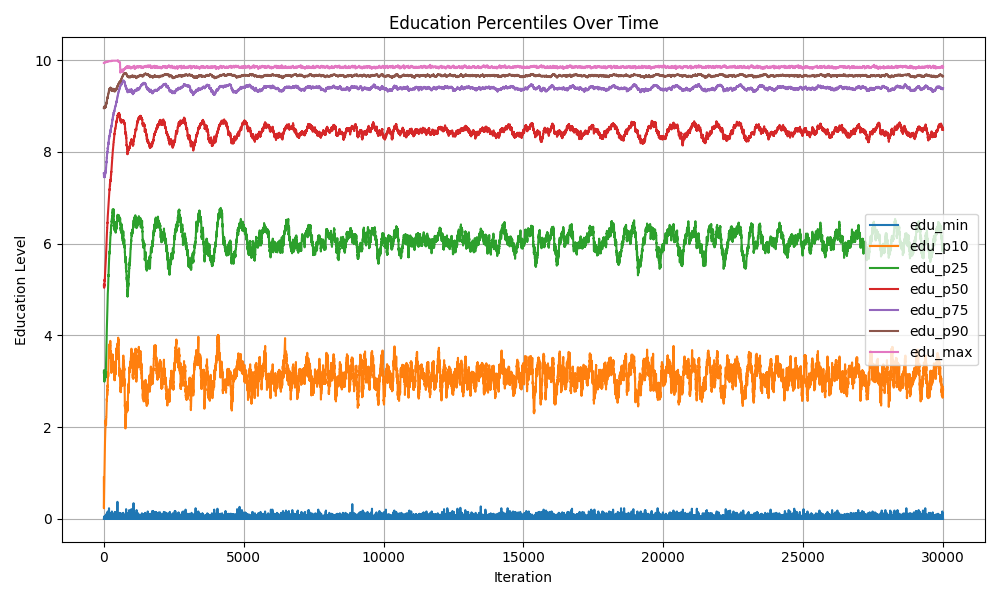
\includegraphics[width=0.48\textwidth]{metrics_config2/metrics_config2_education_perc_time.png}}
\end{center}
\caption{The difference in education level percentiles over iterations between Configuration 1 (left) and Configuration 2 (right)}
\end{figure}

\subsection{Configuration 3: Income and consumption parameters}

\begin{minipage}{0.48\textwidth}
\captionof{listing}{Configuration 0 \& 1 \& 2}
\begin{minted}[fontsize=\small]{json}
{
  // ...
  "income_and_consumption": {
    "income_age_parameter": 0.05,
    "income_education_parameter": 2.0,
    "base_consumption": 10.0,
    "aditional_consumption_rate": 0.2
  },
  // ...
}
\end{minted}
\end{minipage}
\hfill
\begin{minipage}{0.48\textwidth}
\captionof{listing}{Configuration 3}
\begin{minted}[fontsize=\small]{json}
{
  // ...
  "income_and_consumption": {
    "income_age_parameter": 0.15,
    "income_education_parameter": 4.0,
    "base_consumption": 15.0,
    "aditional_consumption_rate": 0.3
  },
  // ...
}
\end{minted}
\end{minipage}

    In this configuration, we modified the parameters responsible for establishing the income in iteration by increasing the education ($\alpha$) and age ($\beta$) parameters and also increasing base and additional consumption.

    The main difference related to these changes is shown in the average amount of money per transaction, which increased about twice, and the total amount of money in transactions over iterations. Moreover, the wealth values of percentiles also increased about twice, but the ratio of percentiles remained the same.

    The side effect of the introduced changes is the increased oscillation time at the beginning of the simulation, which is visible in Fig. \ref{fig:c2-average_transaction_amount} and \ref{fig:c3-average_transaction_amount}.

\begin{figure}[H]
\begin{center}
\subfigure{%
\label{fig:c2-average_transaction_amount}
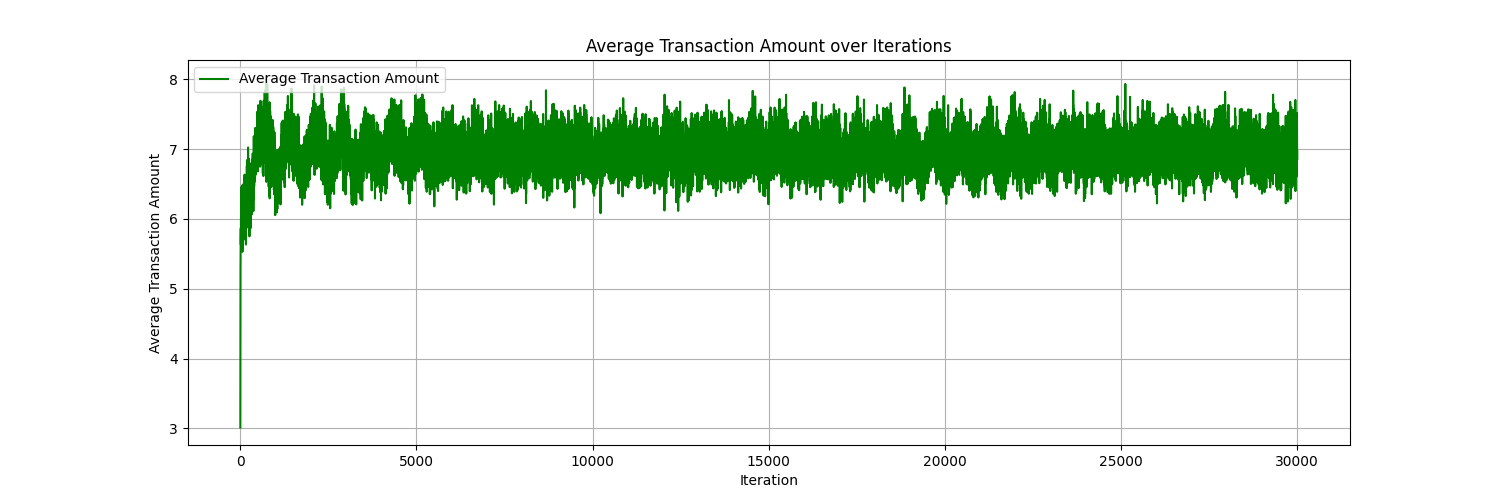
\includegraphics[width=0.48\textwidth]{metrics_config2/metrics_config2_average_transaction_amount.png}}%
\subfigure{%
\label{fig:c3-average_transaction_amount}
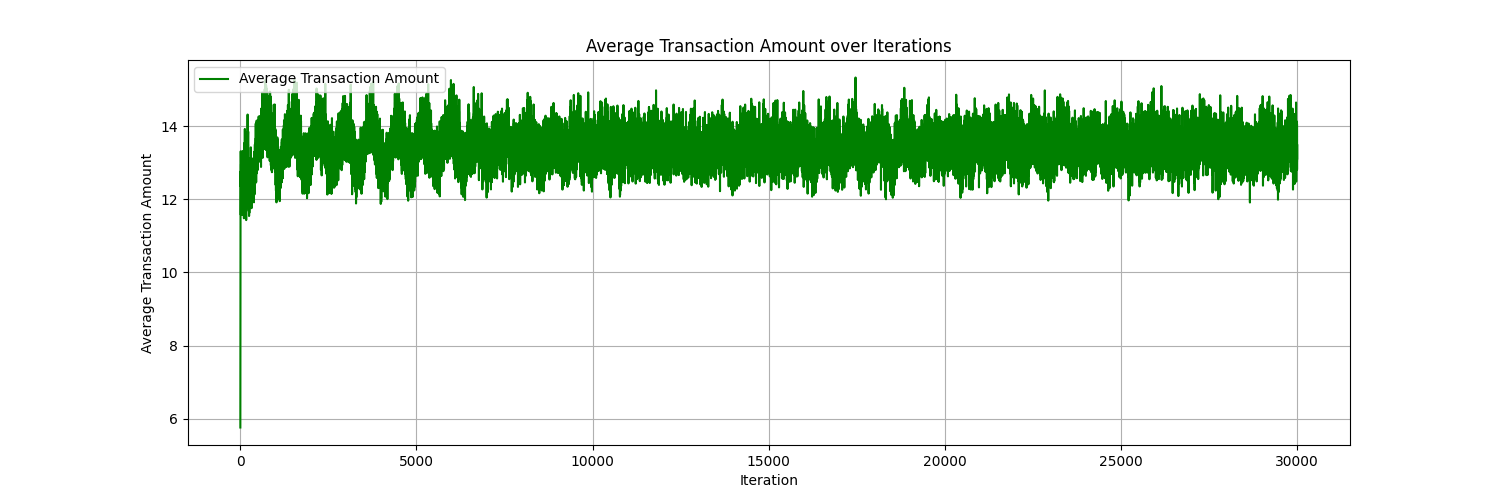
\includegraphics[width=0.48\textwidth]{metrics_config3/metrics_config3_average_transaction_amount.png}}
\end{center}
\caption{The difference in average money amount per transaction over iterations between Configuration 2 (left) and Configuration 3 (right)}
\end{figure}

\begin{figure}[H]
\begin{center}
\subfigure{%
\label{fig:c2-wealth_perc_time}
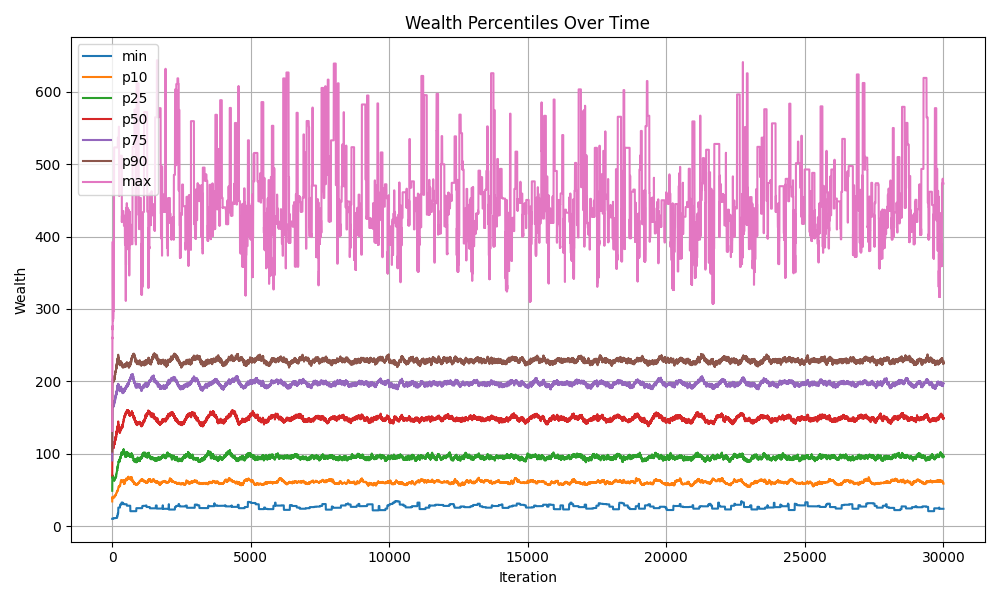
\includegraphics[width=0.48\textwidth]{metrics_config2/metrics_config2_wealth_perc_time.png}}%
\subfigure{%
\label{fig:c3-wealth_perc_time}
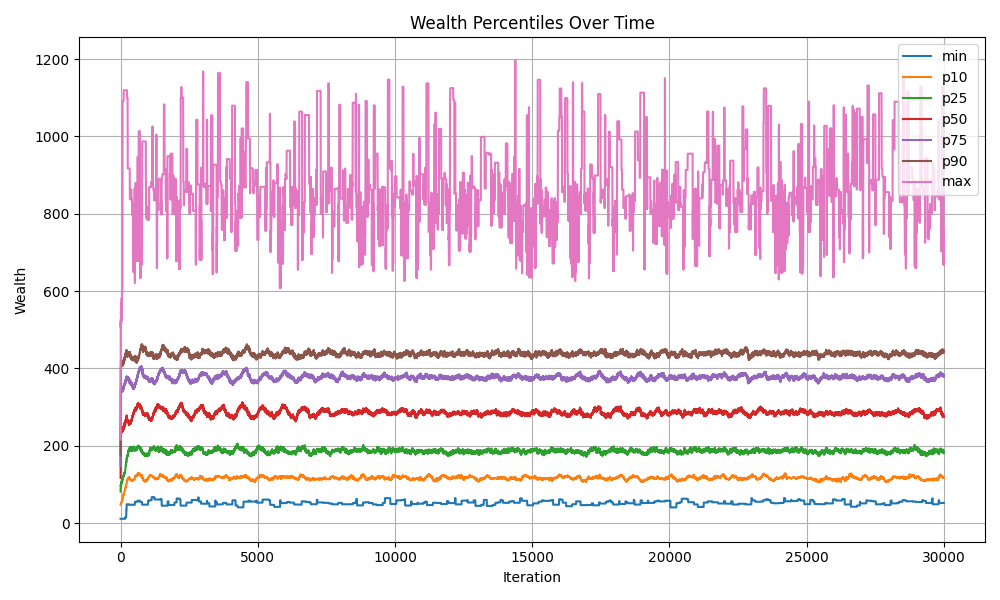
\includegraphics[width=0.48\textwidth]{metrics_config3/metrics_config3_wealth_perc_time.png}}
\end{center}
\caption{The difference in wealth percentiles over iterations between Configuration 2 (left) and Configuration 3 (right)}
\end{figure}

\subsection{Configuration 4: Transactions parameters}

\begin{minipage}{0.48\textwidth}
\captionof{listing}{Configuration 0 \& 1 \& 2 \& 3}
\begin{minted}[fontsize=\small]{json}
{
  // ...
  "transaction": {
    "transaction_probability": 0.3,
    "education_parameter": 1.0,
    "age_parameter": 0.001,
    "tax_rate": 0.05,
    "amount_rate": 0.05
  },
  // ...
}
\end{minted}
\end{minipage}
\hfill
\begin{minipage}{0.48\textwidth}
\captionof{listing}{Configuration 4}
\begin{minted}[fontsize=\small]{json}
{
  // ...
  "transaction": {
    "transaction_probability": 0.7,
    "education_parameter": 1.5,
    "age_parameter": 0.005,
    "tax_rate": 0.15,
    "amount_rate": 0.15
  },
  // ...
}
\end{minted}
\end{minipage}

    This time, we strongly increased the probability of the transactions between agents when they are in the transaction radius. We also increased the education and age parameters responsible for choosing the winner of the transaction and increased taxes and the minimal amount of money per transaction.

    These changes led to a huge increase in the metrics related to the transactions and their amounts of money. Moreover, due to the rise in transaction probability, we can see many more transactions happening per iteration.

    As a side effect, the Gini coefficient also climbed to the range $\sim [0.28, 0.31]$, which means that the society is less equal.

    In the below charts, we present the most significant jumps in transactions-related metrics.

\begin{figure}[H]
\begin{center}
\subfigure{%
\label{fig:c3-total_transactions_amount}
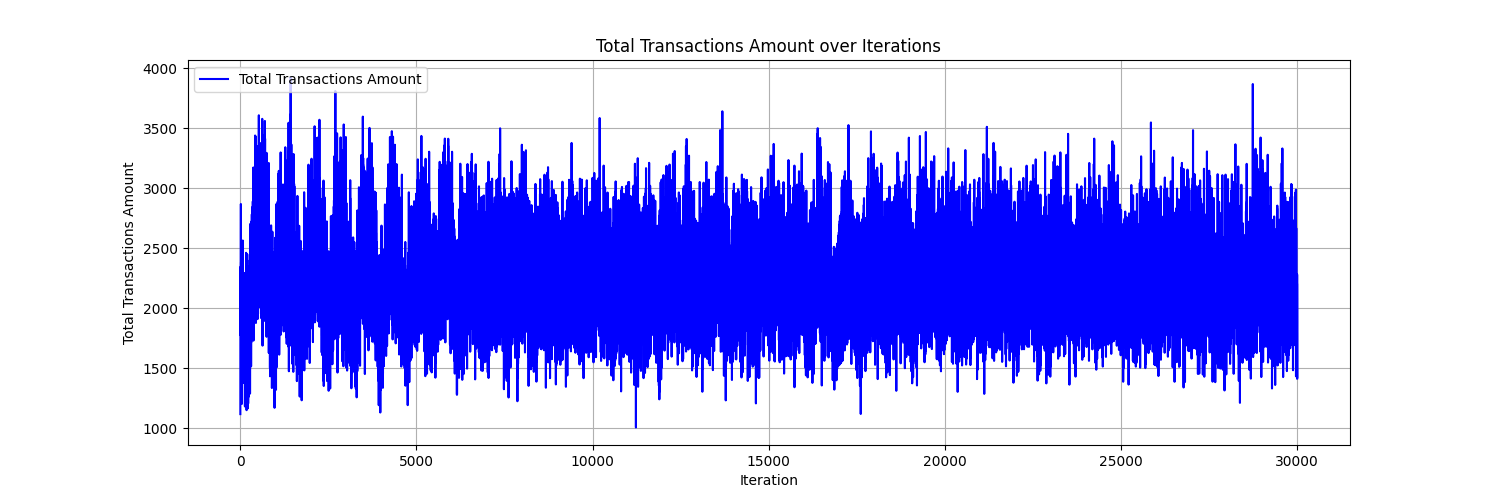
\includegraphics[width=0.48\textwidth]{metrics_config3/metrics_config3_total_transactions_amount.png}}%
\subfigure{%
\label{fig:c4-total_transactions_amount}
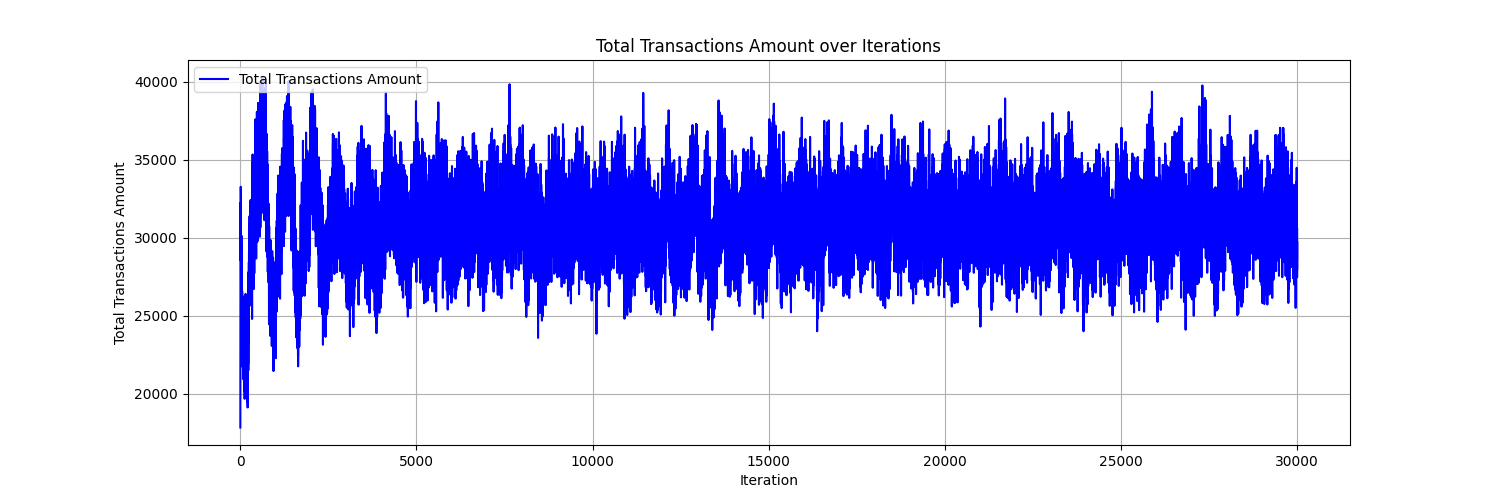
\includegraphics[width=0.48\textwidth]{metrics_config4/metrics_config4_total_transactions_amount.png}}
\end{center}
\caption{The difference in total money amount in transactions over iterations between Configuration 3 (left) and Configuration 4 (right)}
\end{figure}

\begin{figure}[H]
\begin{center}
\subfigure{%
\label{fig:c3-average_transaction_amount}
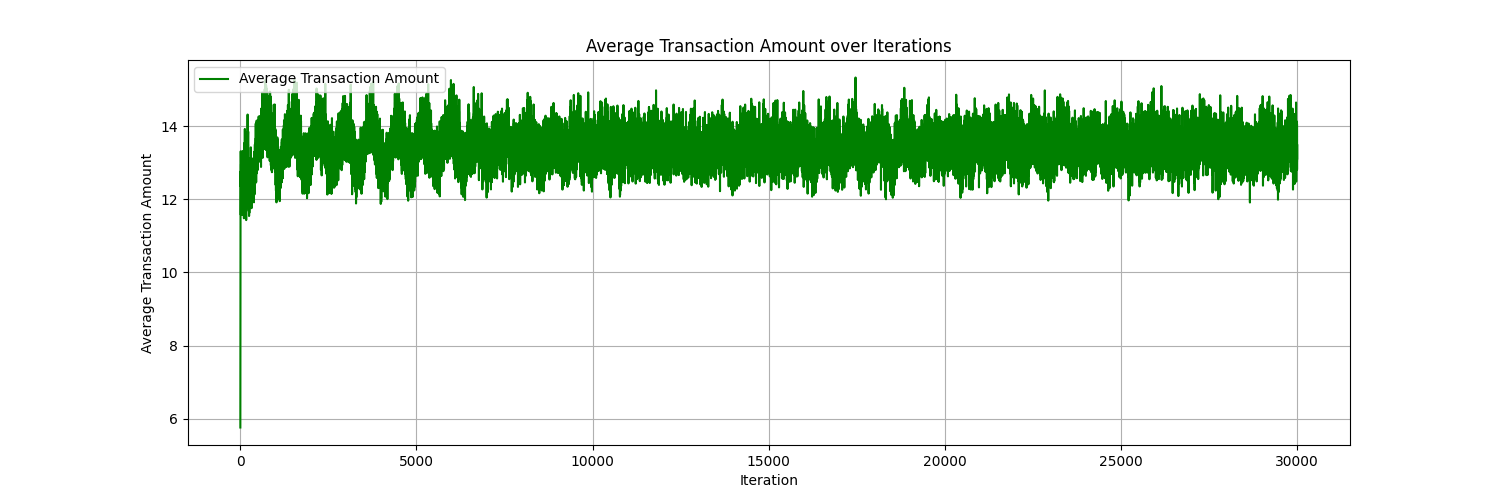
\includegraphics[width=0.48\textwidth]{metrics_config3/metrics_config3_average_transaction_amount.png}}%
\subfigure{%
\label{fig:c4-average_transaction_amount}
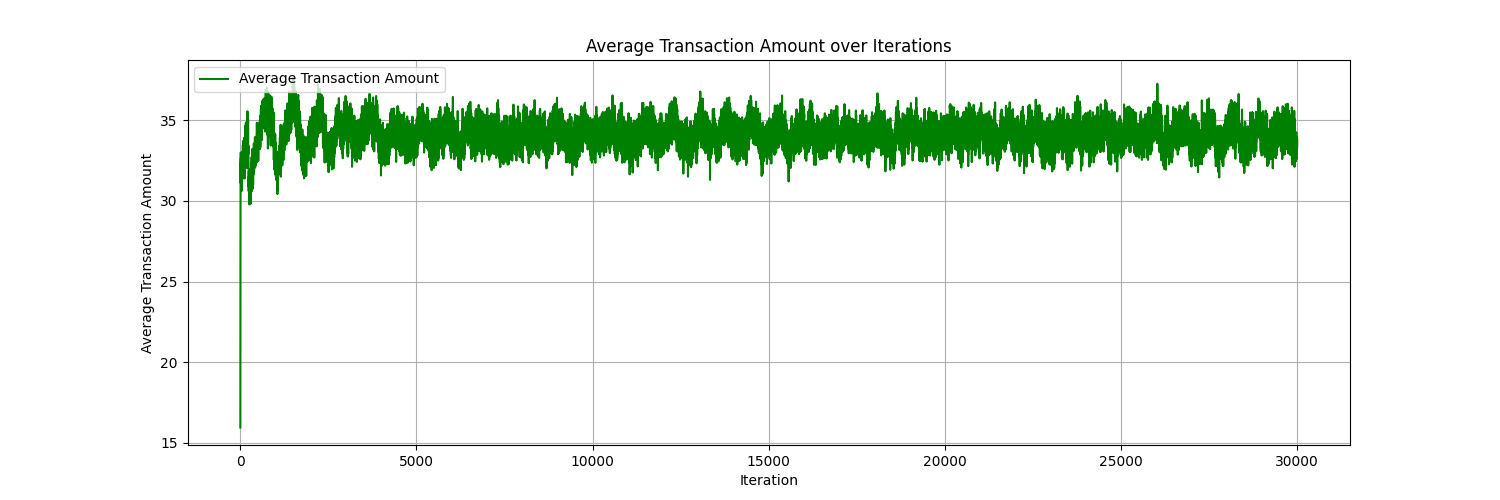
\includegraphics[width=0.48\textwidth]{metrics_config4/metrics_config4_average_transaction_amount.png}}
\end{center}
\caption{The difference in average money amount per transaction over iterations between Configuration 3 (left) and Configuration 4 (right)}
\end{figure}

\begin{figure}[H]
\begin{center}
\subfigure{%
\label{fig:c3-total_transactions_count}
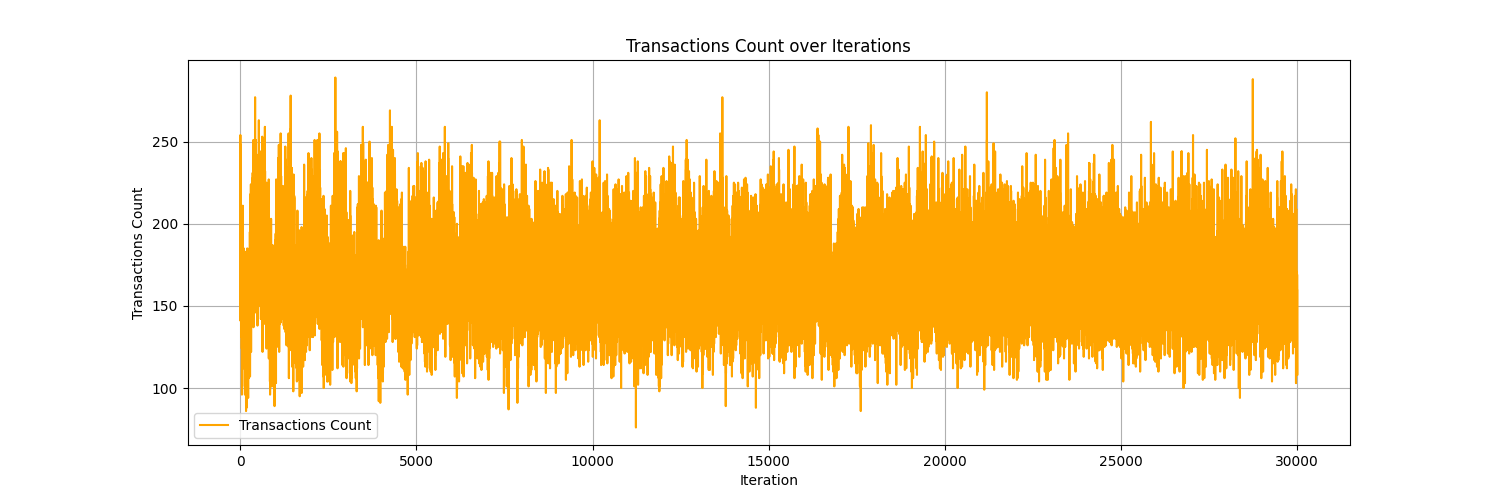
\includegraphics[width=0.48\textwidth]{metrics_config3/metrics_config3_total_transactions_count.png}}%
\subfigure{%
\label{fig:c4-total_transactions_count}
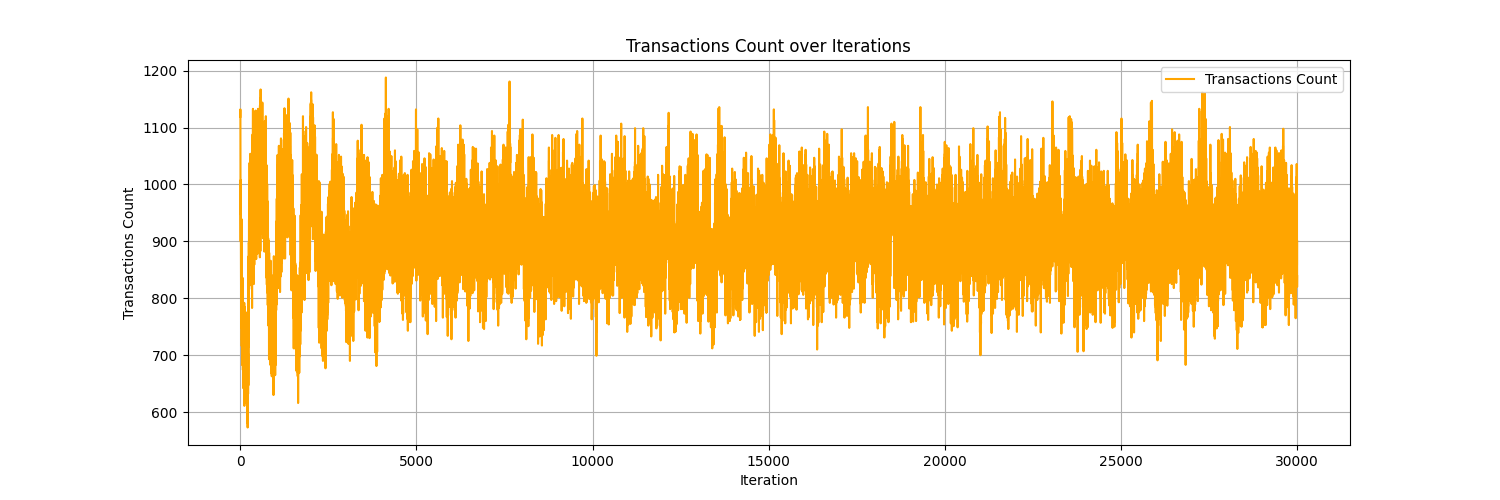
\includegraphics[width=0.48\textwidth]{metrics_config4/metrics_config4_total_transactions_count.png}}
\end{center}
\caption{The difference in total number of transactions (count) over iterations between Configuration 3 (left) and Configuration 4 (right)}
\end{figure}

\subsection{Configuration 5: Wealth parameters}

\begin{minipage}{0.48\textwidth}
\captionof{listing}{Configuration 0 \& 1 \& 2 \& 3 \& 4}
\begin{minted}[fontsize=\small]{json}
{
  // ...
  "wealth": {
    "min_initial_wealth": 10.0,
    "max_initial_wealth": 100.0,
    "min_inheritance_at_birth_rate": 0.1,
    "max_inheritance_at_birth_rate": 0.3
  }
  // ...
}
\end{minted}
\end{minipage}
\hfill
\begin{minipage}{0.48\textwidth}
\captionof{listing}{Configuration 5}
\begin{minted}[fontsize=\small]{json}
{
  // ...
  "wealth": {
    "min_initial_wealth": 10.0,
    "max_initial_wealth": 300.0,
    "min_inheritance_at_birth_rate": 0.1,
    "max_inheritance_at_birth_rate": 0.6
  }
  // ...
}
\end{minted}
\end{minipage}

    In this last configuration change, we expanded the range of possible initial wealth by increasing the maximal value from $100$ to $300$ and we also expanded the range of the inheritance at birth from the maximal rate of $0.3$ to $0.6$.

    This change positively influenced the range of the population's Gini coefficient by reducing it to $\sim [0.25, 0.275]$ and it also increased the maximal wealth over iterations. In addition, it raised the total population's wealth over iterations.

\begin{figure}[H]
\begin{center}
\subfigure{%
\label{fig:c4-gini_coefficient}
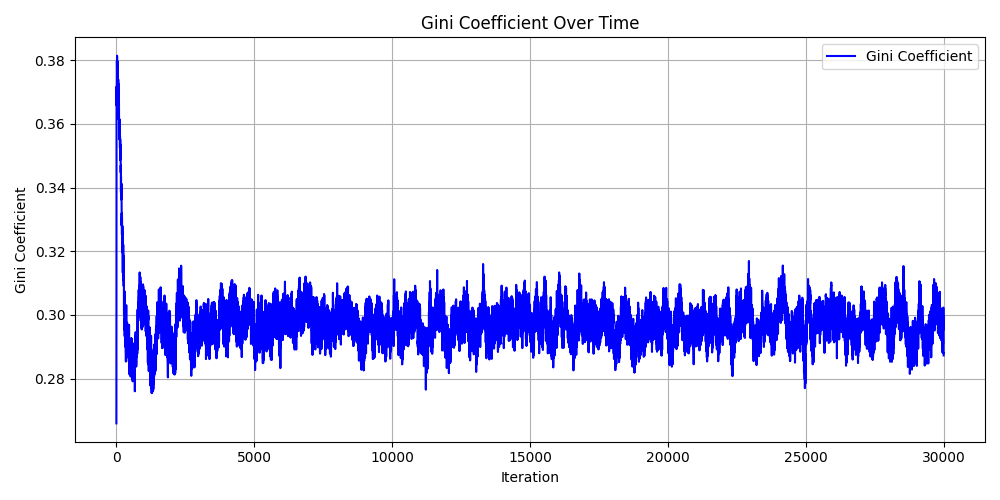
\includegraphics[width=0.48\textwidth]{metrics_config4/metrics_config4_gini_coefficient.png}}%
\subfigure{%
\label{fig:c5-gini_coefficient}
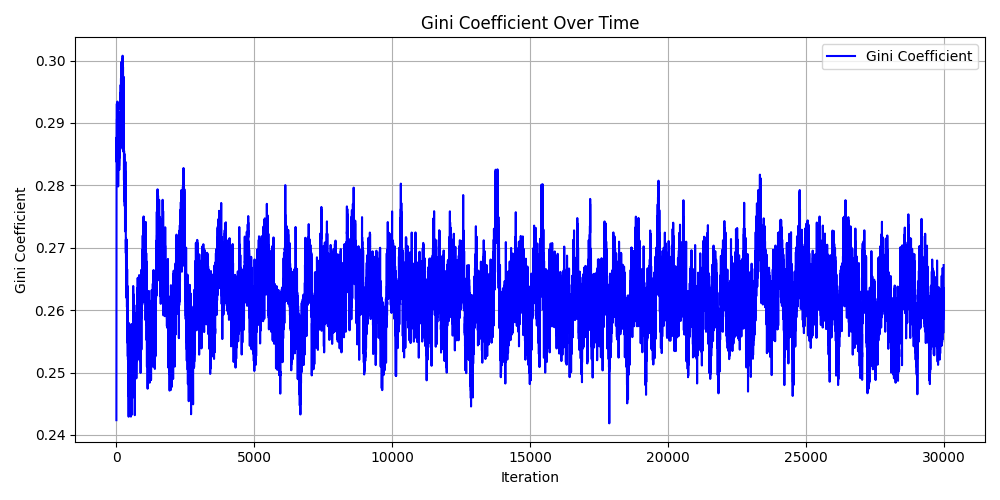
\includegraphics[width=0.48\textwidth]{metrics_config5/metrics_config5_gini_coefficient.png}}
\end{center}
\caption{The difference in population's Gini coefficient over iterations between Configuration 4 (left) and Configuration 5 (right)}
\end{figure}

\begin{figure}[H]
\begin{center}
\subfigure{%
\label{fig:c4-total_wealth}
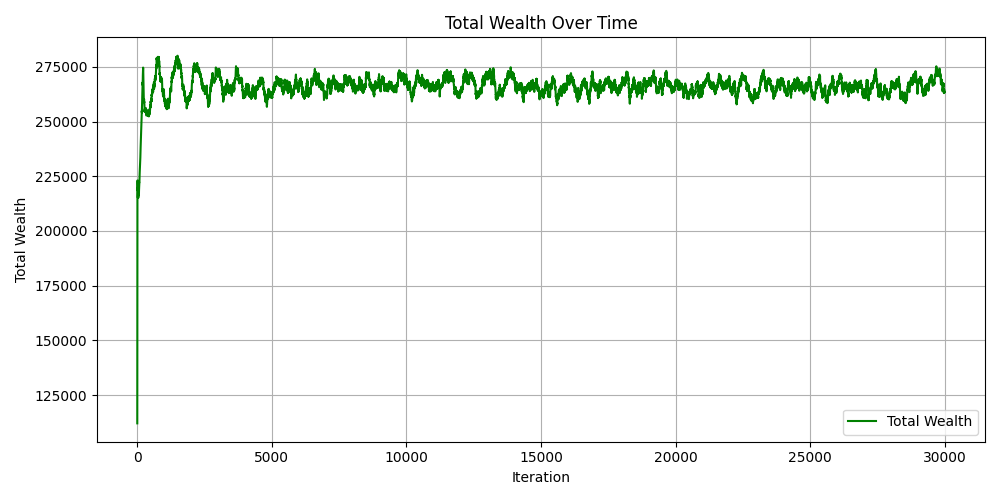
\includegraphics[width=0.48\textwidth]{metrics_config4/metrics_config4_total_wealth.png}}%
\subfigure{%
\label{fig:c5-total_wealth}
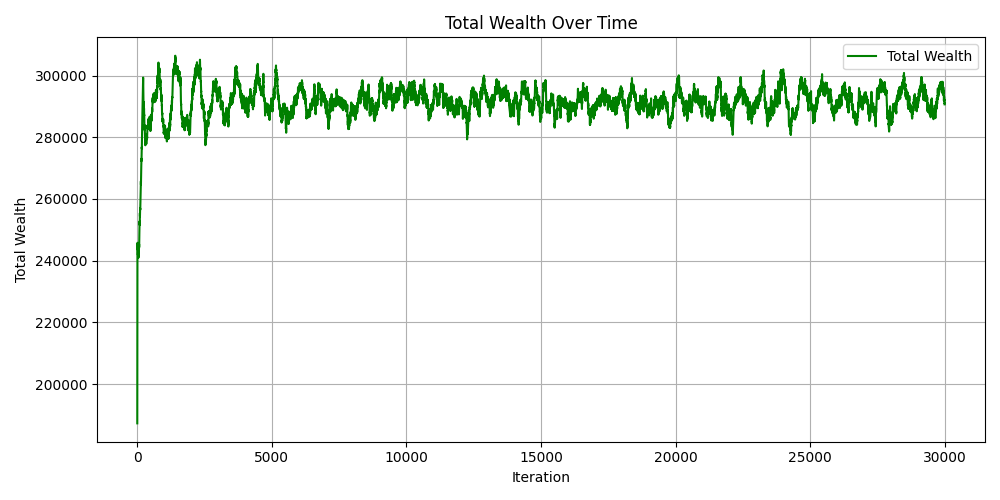
\includegraphics[width=0.48\textwidth]{metrics_config5/metrics_config5_total_wealth.png}}
\end{center}
\caption{The difference in population's total wealth over iterations between Configuration 4 (left) and Configuration 5 (right)}
\end{figure}

\vspace{5mm}

All configurations from \textbf{Configuration 1} to \textbf{Configuration 5} and their visualizations are presented in the \hyperref[sec:appendix]{Appendix}.


% %%%%%%%%%%%%%%%%%%%%%%%%%%%%%%%%%%%%%%%%%%%%%%%%%%%%%%%%%%%%%%%%%%%%%%%%%%%%%%%
% \subsection{Figures and tables}
% \label{sec:figures-tables}

% The text should contain references to all figures and tables used in the paper.

% %%%%%%%%%%%%%%%%%%%%%%%%%%%%%%%%%%%%%%%%%%%%%%%%%%%%%%%%%%%%%%%%%%%%%%%%%%%%%%%
% \subsubsection{Figures}
% \label{sec:figures}

% Examplary reference to Figure~\ref{fig:ex1}.

% \begin{figure}[!htbp]
%   \centering
% \includegraphics[width=.7\textwidth]{example.pdf}
% \caption{Exemplary figure (source: \cite{author2021title})}
% \label{fig:ex1}
% \end{figure}

% In the case of figures, you can refer to individual subfigures (Figure~\ref{fig:sub1} and Figure~\ref{fig:sub2}) and to the entire Figure~\ref{fig:ex2}.

% \begin{figure}[!htbp]
% \begin{center}
% \subfigure[Title 1]{%
% \label{fig:sub1}
% \includegraphics[width=0.48\textwidth]{example.pdf}}%
% \subfigure[Title 2]{%
% \label{fig:sub2}
% \includegraphics[width=0.48\textwidth]{example.pdf}}
% \end{center}
% \caption{Another exemplary figures (source: \cite{author2021title})}
% \label{fig:ex2}
% \end{figure}

% %%%%%%%%%%%%%%%%%%%%%%%%%%%%%%%%%%%%%%%%%%%%%%%%%%%%%%%%%%%%%%%%%%%%%%%%%%%%%%% 
% \subsubsection{Tables}
% \label{sec:tables}

% Exemplary Table~\ref{tab:ex1}.

% \begin{table}[!htbp]
% \centering
% \caption[Exemplary table]{Exemplary table}
% \begin{tabularx}{\columnwidth}{@{}YYYYYYY@{}} \toprule
%   & \multicolumn{2}{c}{\small\textbf{Best}} & \multicolumn{2}{c}{\small\textbf{Average}} & \multicolumn{2}{c}{\small\textbf{Worst}} \\ \cmidrule(lr){2-3} \cmidrule(lr){4-5} \cmidrule(lr){6-7}
%   \textbf{No.} & \textbf{AB} & \textbf{CD} & \textbf{FE} & \textbf{GH} & \textbf{IJ} & \textbf{KL} \\ \midrule
%   \textit{1.} & 10 & 89 & 58 & 244 & 6 & 70 \\  
%   \textit{2.} & 15 & 87 & 57 & 147 & 4 & 82 \\
%   \textit{3.} & 23 & 45 & 55 & 151 & 2 & 38 \\
%   \textit{4.} & 34 & 90 & 55 & 246 & 1 & 82 \\
%   \textit{5.} & 56 & 75 & 54 & 255 & 0 & 73 \\ \bottomrule
% \end{tabularx}
% \label{tab:ex1}
% \end{table}

% %%%%%%%%%%%%%%%%%%%%%%%%%%%%%%%%%%%%%%%%%%%%%%%%%%%%%%%%%%%%%%%%%%%%%%%%%%%%%%%
\section{\SectionTitleSummary}
\label{sec:conclusions}

% % the following content of the section should be removed from the final version of the report.

\emph{Summary of the research results, conclusions and plans for further work.}

The simulation implementation we created proves that simulating a socio-economical system is possible to some extent with selected constraints. In this paper, we showed that a constraint commonly used in related work, that cumulative wealth of a population should be constant, is redundant in an environment with properly tuned parameters. Given examples of several configurations, the total wealth converged over the course of the simulation with negligible noise. 

The wealth distribution tends to be \textit{somewhat} unequal. The 10th, 25th, 50th, 75th, and 90th percentiles along with the minimal wealth converged similarly to the total wealth. However, the maximal wealth was erratic and much larger than the 90th percentile, which indicates right skewness of the wealth distribution. This proves that it was easier to gain wealth for agents that were already wealthy.

Our simulation is far simpler than the real world. The possible further work could be introducing a goods trading system instead of random transactions, which would further nuance the agents' interactions. Another way of improving the simulation might be running several quasi-isolated systems with agents' migrations to simulate multiple villages.

%%%%%%%%%%%%%%%%%%%%%%%%%%%%%%%%%%%%%%%%%%%%%%%%%%%%%%%%%%%%%%%%%%%%%%%%%%%%%%%
\printbibliography

%%%%%%%%%%%%%%%%%%%%%%%%%%%%%%%%%%%%%%%%%%%%%%%%%%%%%%%%%%%%%%%%%%%%%%%%%%%%%%%

\section*{Appendix}
\label{sec:appendix}

\subsection*{Configuration 1}

    \captionof{listing}{Configuration 1 parameters}
    \begin{minted}{json}
{
  "num_iterations": 30000,
  "num_agents": 1000,
  "length": 1500,
  "width": 1500,
  "interaction_radius": 75.0,
  "max_movement": 20.0,
  "age_and_death": {
    "mean_age": 35.0,
    "stddev_age": 15.0,
    "mid_age": 80.0,
    "max_start_age": 70.0,
    "steepness": 0.02
  },
  "education": {
    "initial_adult_min": 4.0,
    "initial_adult_max": 10.0,
    "elemental_education_threshold": 4.0,
    "children_education_jitter": 2.0,
    "learning_rate_min": 0.005,
    "learning_rate_max": 0.05,
    "max": 10.0
  },
  "income_and_consumption": {
    "income_age_parameter": 0.05,
    "income_education_parameter": 2.0,
    "base_consumption": 10.0,
    "aditional_consumption_rate": 0.2
  },
  "transaction": {
    "transaction_probability": 0.3,
    "education_parameter": 1.0,
    "age_parameter": 0.001,
    "tax_rate": 0.05,
    "amount_rate": 0.05
  },
  "wealth": {
    "min_initial_wealth": 10.0,
    "max_initial_wealth": 100.0,
    "min_inheritance_at_birth_rate": 0.1,
    "max_inheritance_at_birth_rate": 0.3
  }
}
    \end{minted}

    The computed metrics in the form of line plots:

    \begin{figure}[H]
        \centering
        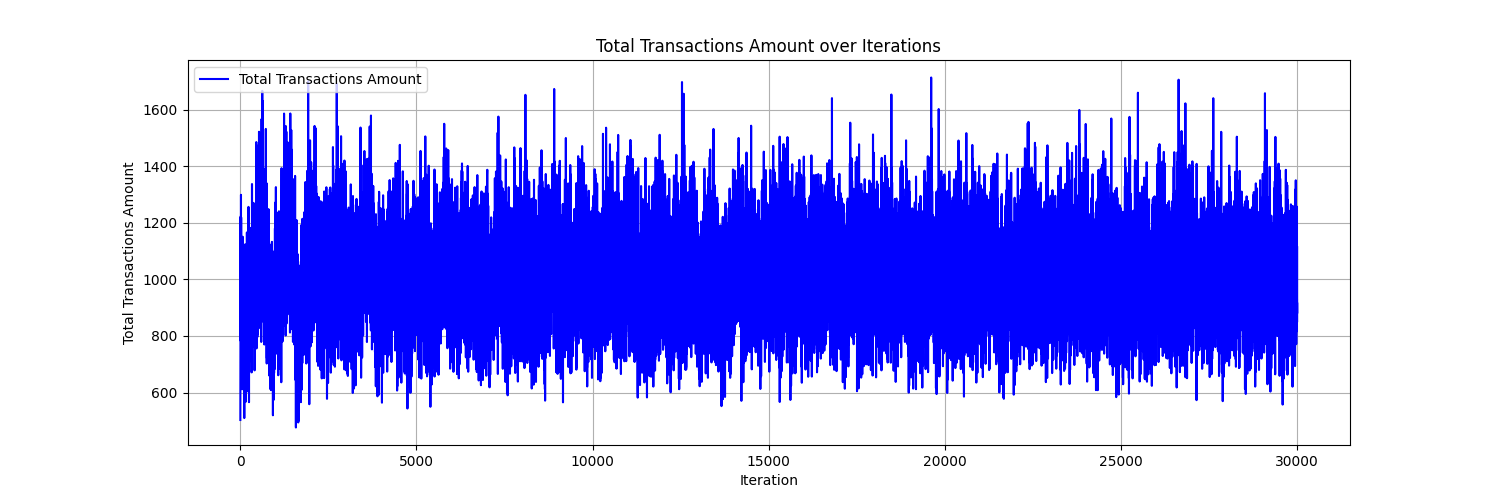
\includegraphics[width=0.8\linewidth]{metrics_config1/metrics_config1_total_transactions_amount.png}
        \caption{Configuration 1: Total transactions' amount over iterations}
        \label{fig:c0-total_transactions_amount}
    \end{figure}

    \begin{figure}[H]
        \centering
        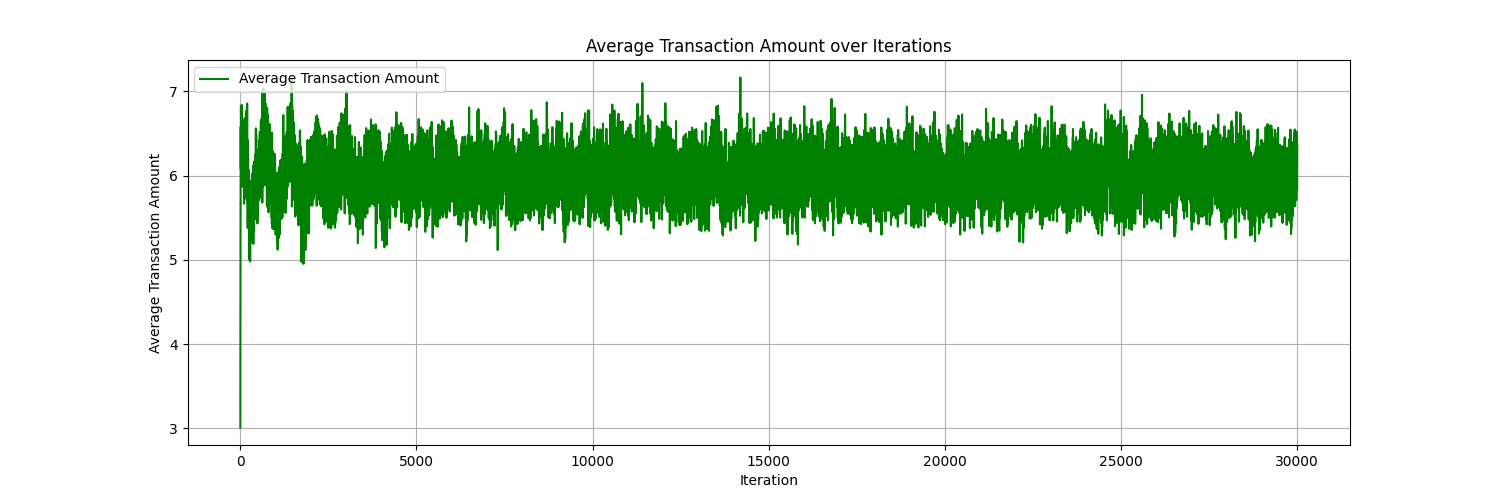
\includegraphics[width=0.8\linewidth]{metrics_config1/metrics_config1_average_transaction_amount.png}
        \caption{Configuration 1: Average transaction amount over iterations}
        \label{fig:c0-average_transaction_amount}
    \end{figure}

    \begin{figure}[H]
        \centering
        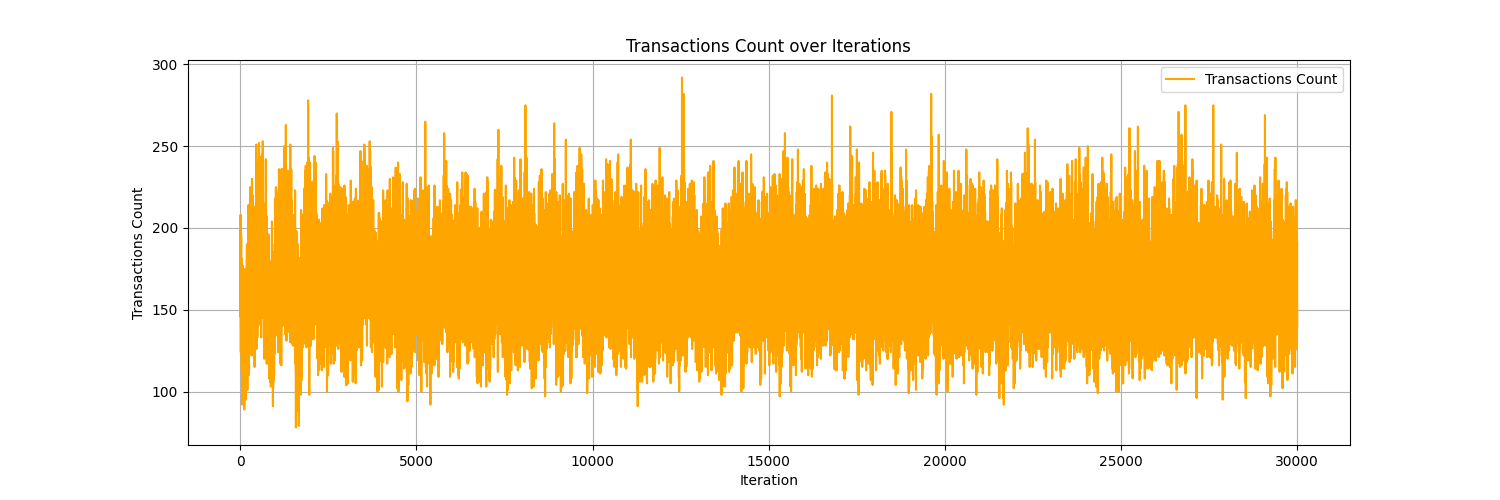
\includegraphics[width=0.8\linewidth]{metrics_config1/metrics_config1_total_transactions_count.png}
        \caption{Configuration 1: Total number of transactions (count) over iterations}
        \label{fig:c0-total_transactions_count}
    \end{figure}

    \begin{figure}[H]
        \centering
        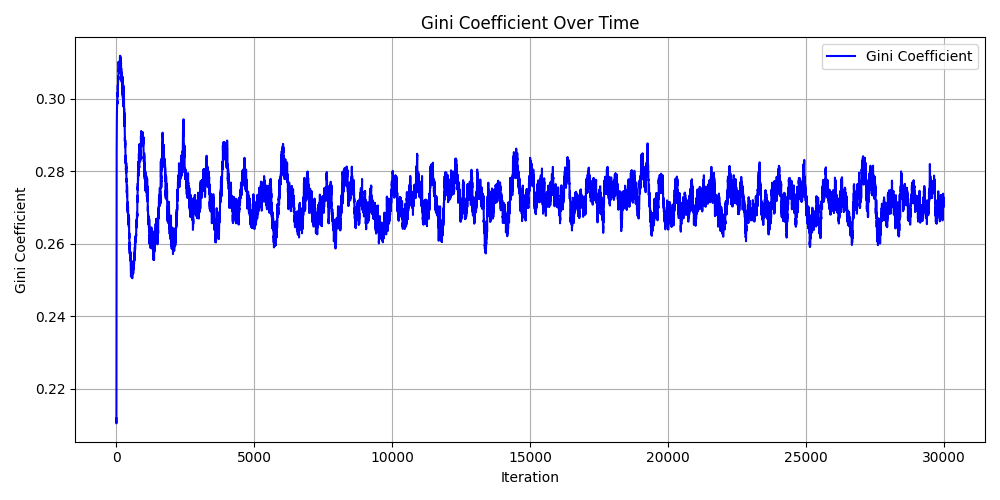
\includegraphics[width=0.8\linewidth]{metrics_config1/metrics_config1_gini_coefficient.png}
        \caption{Configuration 1: Gini coefficient of population's wealth over iterations}
        \label{fig:c0-gini_coefficient}
    \end{figure}

    \begin{figure}[H]
        \centering
        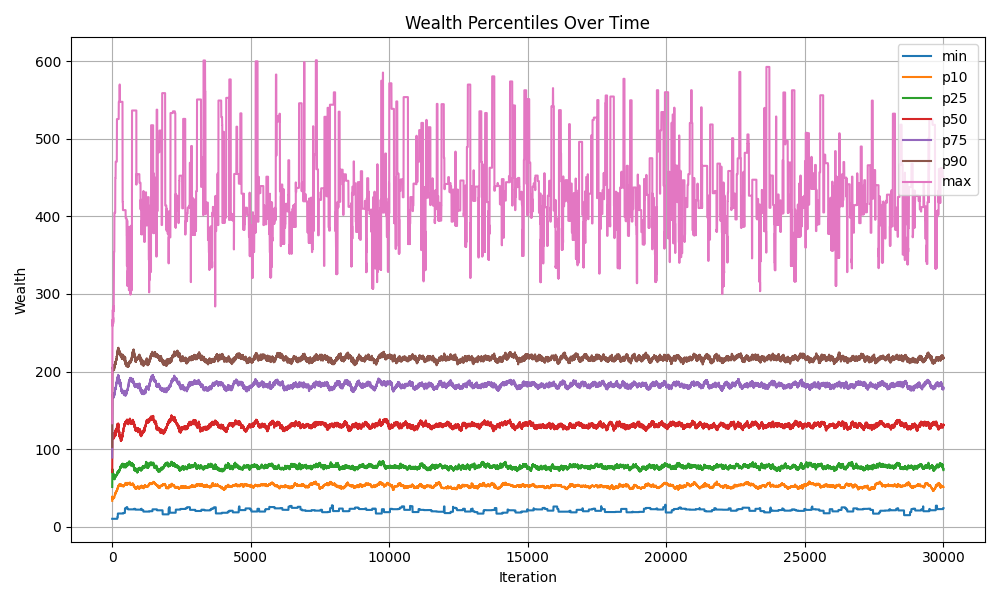
\includegraphics[width=0.8\linewidth]{metrics_config1/metrics_config1_wealth_perc_time.png}
        \caption{Configuration 1: Population's wealth percentiles over iterations}
        \label{fig:c0-wealth_perc_time}
    \end{figure}

    \begin{figure}[H]
        \centering
        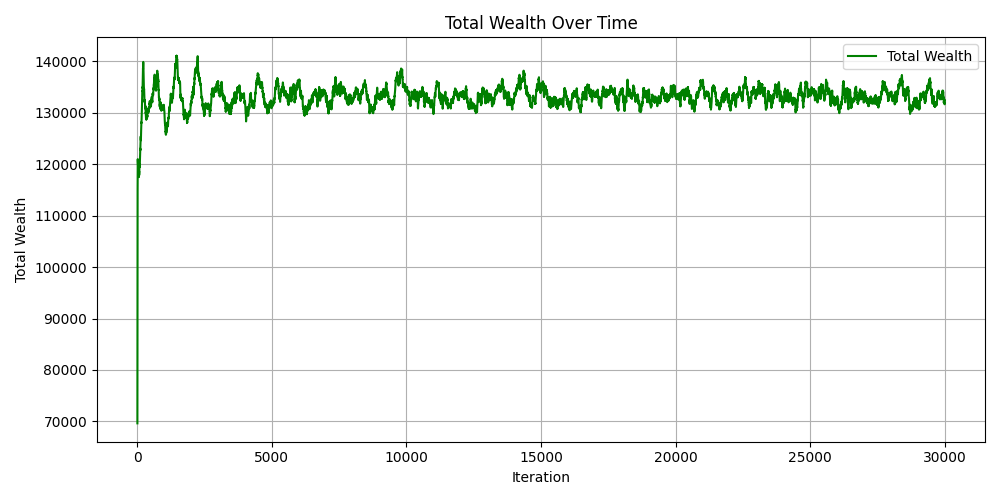
\includegraphics[width=0.8\linewidth]{metrics_config1/metrics_config1_total_wealth.png}
        \caption{Configuration 1: Total population's wealth over iterations}
        \label{fig:c0-total_wealth}
    \end{figure}

    \begin{figure}[H]
        \centering
        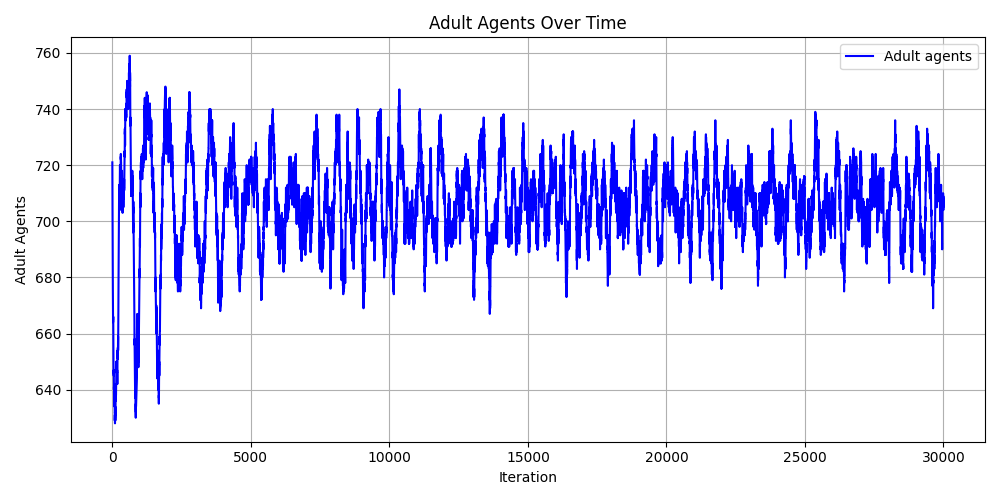
\includegraphics[width=0.8\linewidth]{metrics_config1/metrics_config1_adult_agents.png}
        \caption{Configuration 1: Number of adult agents over iterations}
        \label{fig:c0-adult_agents}
    \end{figure}

    \begin{figure}[H]
        \centering
        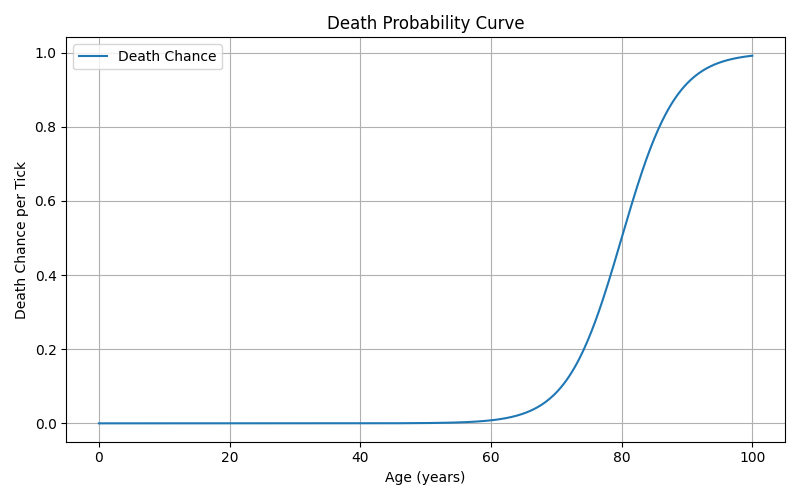
\includegraphics[width=0.8\linewidth]{metrics_config1/metrics_config1_death_probability_curve.png}
        \caption{Configuration 1: Death probability curve}
        \label{fig:c0-death_probability_curve}
    \end{figure}

    \begin{figure}[H]
        \centering
        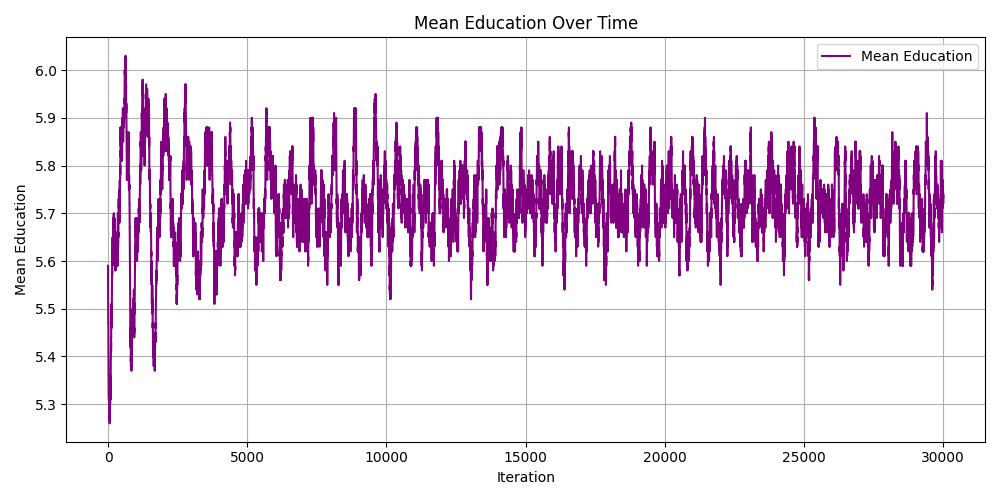
\includegraphics[width=0.8\linewidth]{metrics_config1/metrics_config1_mean_education.png}
        \caption{Configuration 1: Mean education level over iterations}
        \label{fig:c0-mean_education}
    \end{figure}

    \begin{figure}[H]
        \centering
        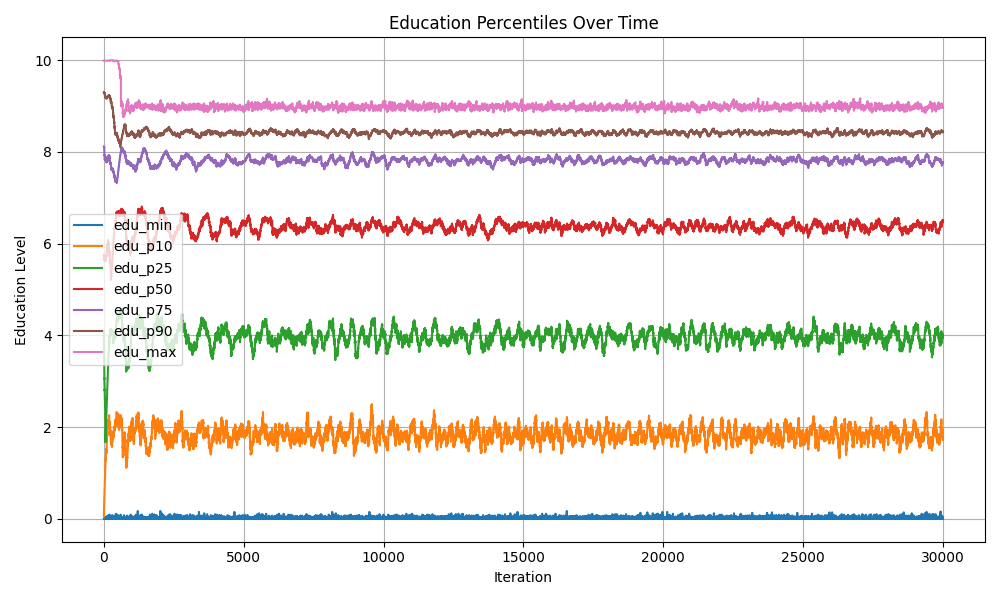
\includegraphics[width=0.8\linewidth]{metrics_config1/metrics_config1_education_perc_time.png}
        \caption{Configuration 1: Education level percentiles over iterations}
        \label{fig:c0-education_perc_time}
    \end{figure}

\subsection*{Configuration 2}

    \captionof{listing}{Configuration 2 parameters}
    \begin{minted}{json}
{
  "num_iterations": 30000,
  "num_agents": 1000,
  "length": 1500,
  "width": 1500,
  "interaction_radius": 75.0,
  "max_movement": 20.0,
  "age_and_death": {
    "mean_age": 35.0,
    "stddev_age": 15.0,
    "mid_age": 80.0,
    "max_start_age": 70.0,
    "steepness": 0.02
  },
  "education": {
    "initial_adult_min": 3.0,
    "initial_adult_max": 10.0,
    "elemental_education_threshold": 3.0,
    "children_education_jitter": 2.0,
    "learning_rate_min": 0.001,
    "learning_rate_max": 0.1,
    "max": 10.0
  },
  "income_and_consumption": {
    "income_age_parameter": 0.05,
    "income_education_parameter": 2.0,
    "base_consumption": 10.0,
    "aditional_consumption_rate": 0.2
  },
  "transaction": {
    "transaction_probability": 0.3,
    "education_parameter": 1.0,
    "age_parameter": 0.001,
    "tax_rate": 0.05,
    "amount_rate": 0.05
  },
  "wealth": {
    "min_initial_wealth": 10.0,
    "max_initial_wealth": 100.0,
    "min_inheritance_at_birth_rate": 0.1,
    "max_inheritance_at_birth_rate": 0.3
  }
}
    \end{minted}

    The computed metrics in the form of line plots:

    \begin{figure}[H]
        \centering
        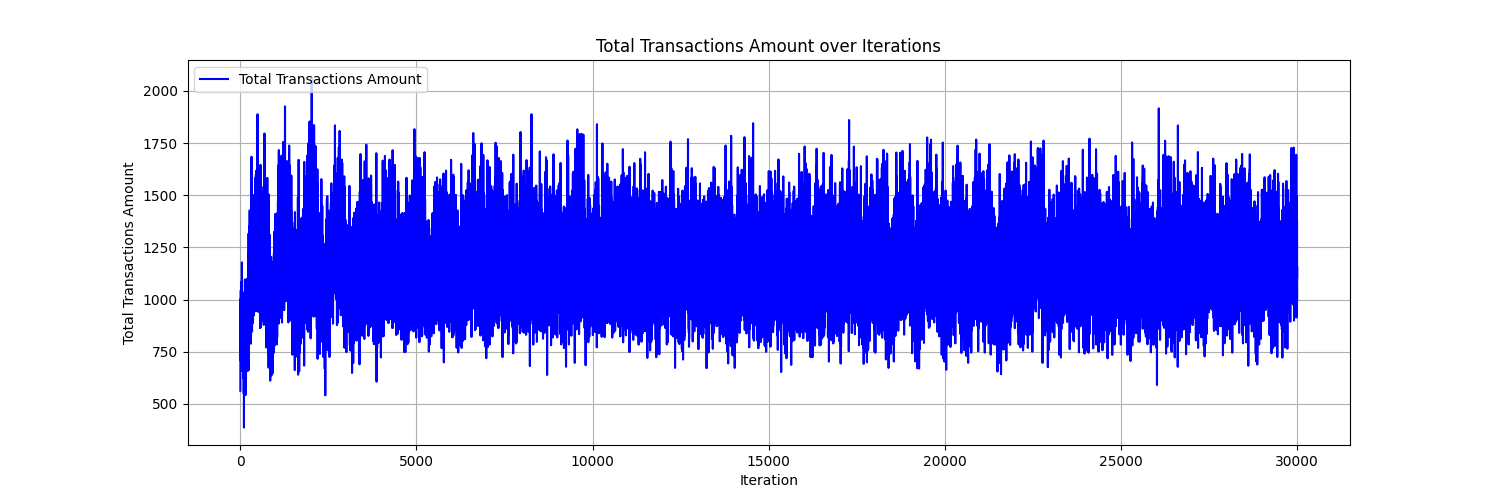
\includegraphics[width=0.8\linewidth]{metrics_config2/metrics_config2_total_transactions_amount.png}
        \caption{Configuration 2: Total transactions' amount over iterations}
        \label{fig:c0-total_transactions_amount}
    \end{figure}

    \begin{figure}[H]
        \centering
        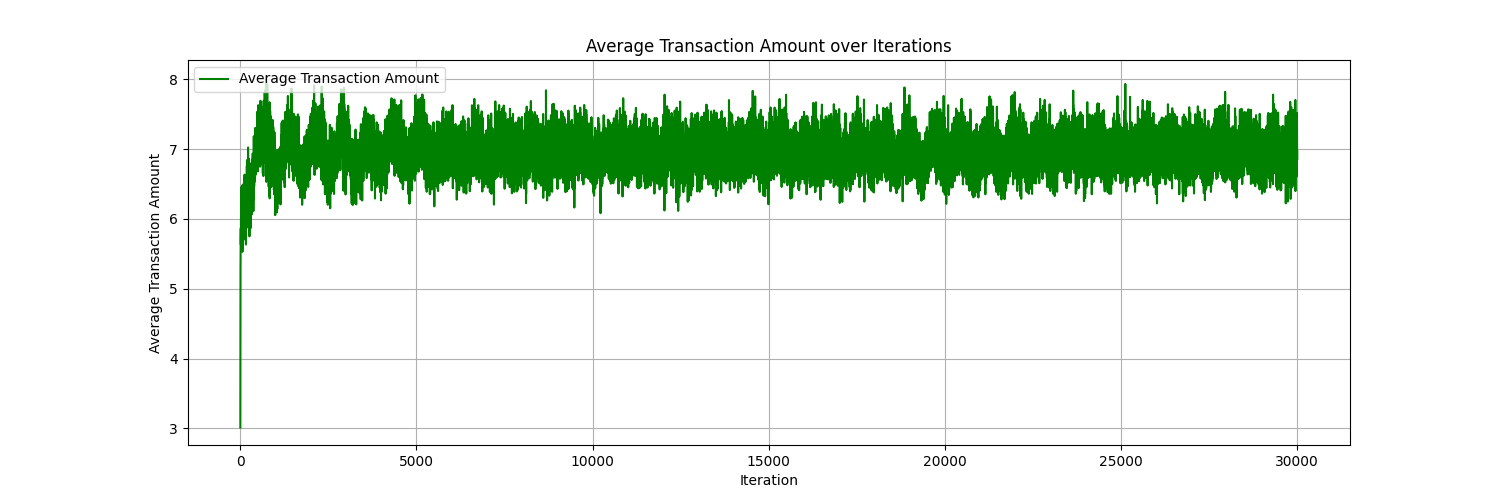
\includegraphics[width=0.8\linewidth]{metrics_config2/metrics_config2_average_transaction_amount.png}
        \caption{Configuration 2: Average transaction amount over iterations}
        \label{fig:c0-average_transaction_amount}
    \end{figure}

    \begin{figure}[H]
        \centering
        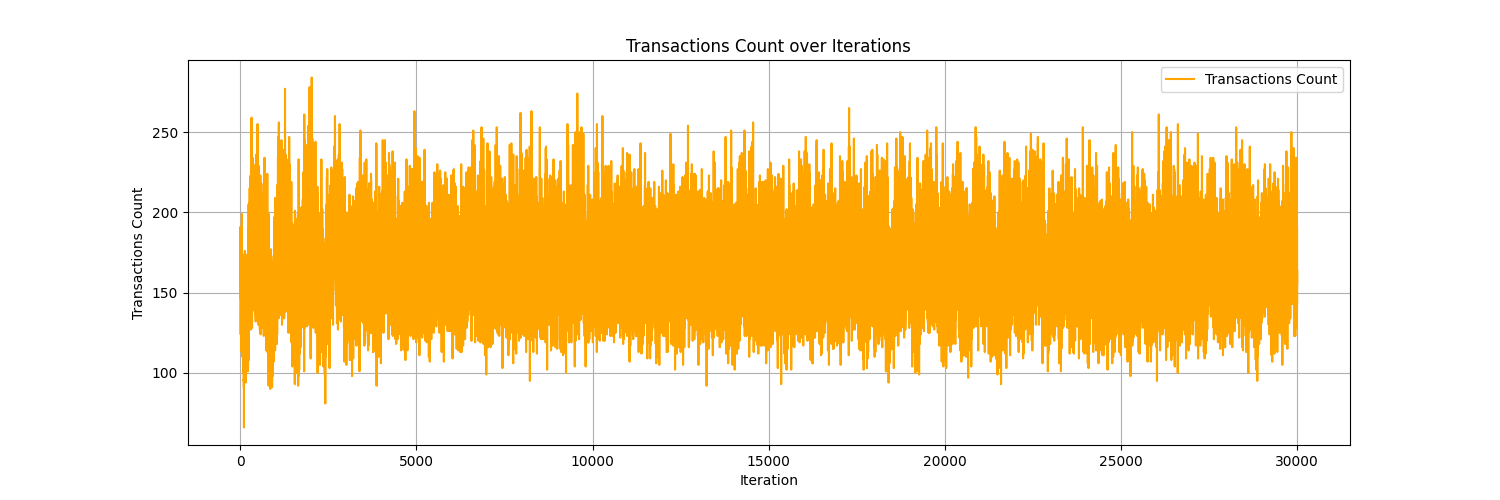
\includegraphics[width=0.8\linewidth]{metrics_config2/metrics_config2_total_transactions_count.png}
        \caption{Configuration 2: Total number of transactions (count) over iterations}
        \label{fig:c0-total_transactions_count}
    \end{figure}

    \begin{figure}[H]
        \centering
        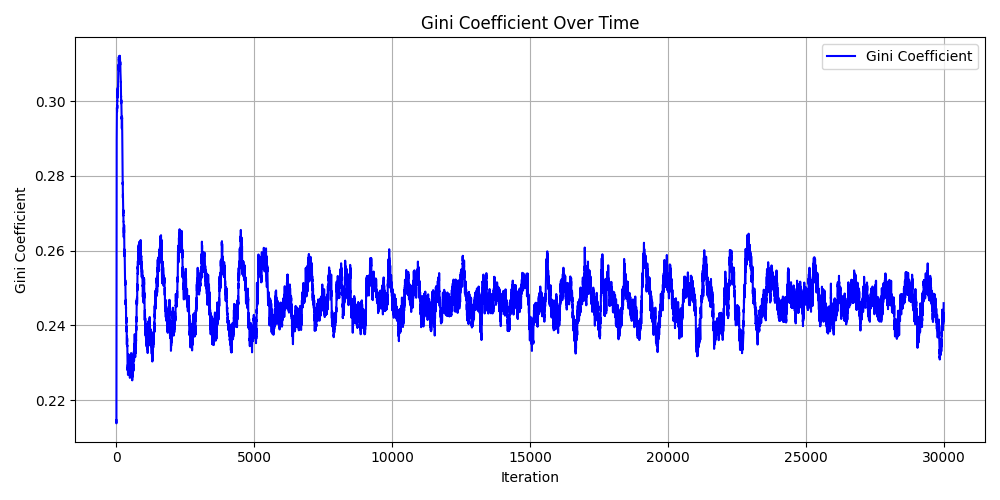
\includegraphics[width=0.8\linewidth]{metrics_config2/metrics_config2_gini_coefficient.png}
        \caption{Configuration 2: Gini coefficient of population's wealth over iterations}
        \label{fig:c0-gini_coefficient}
    \end{figure}

    \begin{figure}[H]
        \centering
        \includegraphics[width=0.8\linewidth]{metrics_config2/metrics_config2_wealth_perc_time.png}
        \caption{Configuration 2: Population's wealth percentiles over iterations}
        \label{fig:c0-wealth_perc_time}
    \end{figure}

    \begin{figure}[H]
        \centering
        \includegraphics[width=0.8\linewidth]{metrics_config2/metrics_config2_total_wealth.png}
        \caption{Configuration 2: Total population's wealth over iterations}
        \label{fig:c0-total_wealth}
    \end{figure}

    \begin{figure}[H]
        \centering
        \includegraphics[width=0.8\linewidth]{metrics_config2/metrics_config2_adult_agents.png}
        \caption{Configuration 2: Number of adult agents over iterations}
        \label{fig:c0-adult_agents}
    \end{figure}

    \begin{figure}[H]
        \centering
        \includegraphics[width=0.8\linewidth]{metrics_config2/metrics_config2_death_probability_curve.png}
        \caption{Configuration 2: Death probability curve}
        \label{fig:c0-death_probability_curve}
    \end{figure}

    \begin{figure}[H]
        \centering
        \includegraphics[width=0.8\linewidth]{metrics_config2/metrics_config2_mean_education.png}
        \caption{Configuration 2: Mean education level over iterations}
        \label{fig:c0-mean_education}
    \end{figure}

    \begin{figure}[H]
        \centering
        \includegraphics[width=0.8\linewidth]{metrics_config2/metrics_config2_education_perc_time.png}
        \caption{Configuration 2: Education level percentiles over iterations}
        \label{fig:c0-education_perc_time}
    \end{figure}

\subsection*{Configuration 3}

    \captionof{listing}{Configuration 3 parameters}
    \begin{minted}{json}
{
  "num_iterations": 30000,
  "num_agents": 1000,
  "length": 1500,
  "width": 1500,
  "interaction_radius": 75.0,
  "max_movement": 20.0,
  "age_and_death": {
    "mean_age": 35.0,
    "stddev_age": 15.0,
    "mid_age": 80.0,
    "max_start_age": 70.0,
    "steepness": 0.02
  },
  "education": {
    "initial_adult_min": 3.0,
    "initial_adult_max": 10.0,
    "elemental_education_threshold": 3.0,
    "children_education_jitter": 2.0,
    "learning_rate_min": 0.001,
    "learning_rate_max": 0.1,
    "max": 10.0
  },
  "income_and_consumption": {
    "income_age_parameter": 0.15,
    "income_education_parameter": 4.0,
    "base_consumption": 15.0,
    "aditional_consumption_rate": 0.3
  },
  "transaction": {
    "transaction_probability": 0.3,
    "education_parameter": 1.0,
    "age_parameter": 0.001,
    "tax_rate": 0.05,
    "amount_rate": 0.05
  },
  "wealth": {
    "min_initial_wealth": 10.0,
    "max_initial_wealth": 100.0,
    "min_inheritance_at_birth_rate": 0.1,
    "max_inheritance_at_birth_rate": 0.3
  }
}
    \end{minted}

    The computed metrics in the form of line plots:

    \begin{figure}[H]
        \centering
        \includegraphics[width=0.8\linewidth]{metrics_config3/metrics_config3_total_transactions_amount.png}
        \caption{Configuration 3: Total transactions' amount over iterations}
        \label{fig:c0-total_transactions_amount}
    \end{figure}

    \begin{figure}[H]
        \centering
        \includegraphics[width=0.8\linewidth]{metrics_config3/metrics_config3_average_transaction_amount.png}
        \caption{Configuration 3: Average transaction amount over iterations}
        \label{fig:c0-average_transaction_amount}
    \end{figure}

    \begin{figure}[H]
        \centering
        \includegraphics[width=0.8\linewidth]{metrics_config3/metrics_config3_total_transactions_count.png}
        \caption{Configuration 3: Total number of transactions (count) over iterations}
        \label{fig:c0-total_transactions_count}
    \end{figure}

    \begin{figure}[H]
        \centering
        \includegraphics[width=0.8\linewidth]{metrics_config3/metrics_config3_gini_coefficient.png}
        \caption{Configuration 3: Gini coefficient of population's wealth over iterations}
        \label{fig:c0-gini_coefficient}
    \end{figure}

    \begin{figure}[H]
        \centering
        \includegraphics[width=0.8\linewidth]{metrics_config3/metrics_config3_wealth_perc_time.png}
        \caption{Configuration 3: Population's wealth percentiles over iterations}
        \label{fig:c0-wealth_perc_time}
    \end{figure}

    \begin{figure}[H]
        \centering
        \includegraphics[width=0.8\linewidth]{metrics_config3/metrics_config3_total_wealth.png}
        \caption{Configuration 3: Total population's wealth over iterations}
        \label{fig:c0-total_wealth}
    \end{figure}

    \begin{figure}[H]
        \centering
        \includegraphics[width=0.8\linewidth]{metrics_config3/metrics_config3_adult_agents.png}
        \caption{Configuration 3: Number of adult agents over iterations}
        \label{fig:c0-adult_agents}
    \end{figure}

    \begin{figure}[H]
        \centering
        \includegraphics[width=0.8\linewidth]{metrics_config3/metrics_config3_death_probability_curve.png}
        \caption{Configuration 3: Death probability curve}
        \label{fig:c0-death_probability_curve}
    \end{figure}

    \begin{figure}[H]
        \centering
        \includegraphics[width=0.8\linewidth]{metrics_config3/metrics_config3_mean_education.png}
        \caption{Configuration 3: Mean education level over iterations}
        \label{fig:c0-mean_education}
    \end{figure}

    \begin{figure}[H]
        \centering
        \includegraphics[width=0.8\linewidth]{metrics_config3/metrics_config3_education_perc_time.png}
        \caption{Configuration 3: Education level percentiles over iterations}
        \label{fig:c0-education_perc_time}
    \end{figure}

\subsection*{Configuration 4}

    \captionof{listing}{Configuration 4 parameters}
    \begin{minted}{json}
{
  "num_iterations": 30000,
  "num_agents": 1000,
  "length": 1500,
  "width": 1500,
  "interaction_radius": 75.0,
  "max_movement": 20.0,
  "age_and_death": {
    "mean_age": 35.0,
    "stddev_age": 15.0,
    "mid_age": 80.0,
    "max_start_age": 70.0,
    "steepness": 0.02
  },
  "education": {
    "initial_adult_min": 3.0,
    "initial_adult_max": 10.0,
    "elemental_education_threshold": 3.0,
    "children_education_jitter": 2.0,
    "learning_rate_min": 0.001,
    "learning_rate_max": 0.1,
    "max": 10.0
  },
  "income_and_consumption": {
    "income_age_parameter": 0.15,
    "income_education_parameter": 4.0,
    "base_consumption": 15.0,
    "aditional_consumption_rate": 0.3
  },
  "transaction": {
    "transaction_probability": 0.7,
    "education_parameter": 1.5,
    "age_parameter": 0.005,
    "tax_rate": 0.15,
    "amount_rate": 0.15
  },
  "wealth": {
    "min_initial_wealth": 10.0,
    "max_initial_wealth": 100.0,
    "min_inheritance_at_birth_rate": 0.1,
    "max_inheritance_at_birth_rate": 0.3
  }
}
    \end{minted}

    The computed metrics in the form of line plots:

    \begin{figure}[H]
        \centering
        \includegraphics[width=0.8\linewidth]{metrics_config4/metrics_config4_total_transactions_amount.png}
        \caption{Configuration 4: Total transactions' amount over iterations}
        \label{fig:c0-total_transactions_amount}
    \end{figure}

    \begin{figure}[H]
        \centering
        \includegraphics[width=0.8\linewidth]{metrics_config4/metrics_config4_average_transaction_amount.png}
        \caption{Configuration 4: Average transaction amount over iterations}
        \label{fig:c0-average_transaction_amount}
    \end{figure}

    \begin{figure}[H]
        \centering
        \includegraphics[width=0.8\linewidth]{metrics_config4/metrics_config4_total_transactions_count.png}
        \caption{Configuration 4: Total number of transactions (count) over iterations}
        \label{fig:c0-total_transactions_count}
    \end{figure}

    \begin{figure}[H]
        \centering
        \includegraphics[width=0.8\linewidth]{metrics_config4/metrics_config4_gini_coefficient.png}
        \caption{Configuration 4: Gini coefficient of population's wealth over iterations}
        \label{fig:c0-gini_coefficient}
    \end{figure}

    \begin{figure}[H]
        \centering
        \includegraphics[width=0.8\linewidth]{metrics_config4/metrics_config4_wealth_perc_time.png}
        \caption{Configuration 4: Population's wealth percentiles over iterations}
        \label{fig:c0-wealth_perc_time}
    \end{figure}

    \begin{figure}[H]
        \centering
        \includegraphics[width=0.8\linewidth]{metrics_config4/metrics_config4_total_wealth.png}
        \caption{Configuration 4: Total population's wealth over iterations}
        \label{fig:c0-total_wealth}
    \end{figure}

    \begin{figure}[H]
        \centering
        \includegraphics[width=0.8\linewidth]{metrics_config4/metrics_config4_adult_agents.png}
        \caption{Configuration 4: Number of adult agents over iterations}
        \label{fig:c0-adult_agents}
    \end{figure}

    \begin{figure}[H]
        \centering
        \includegraphics[width=0.8\linewidth]{metrics_config4/metrics_config4_death_probability_curve.png}
        \caption{Configuration 4: Death probability curve}
        \label{fig:c0-death_probability_curve}
    \end{figure}

    \begin{figure}[H]
        \centering
        \includegraphics[width=0.8\linewidth]{metrics_config4/metrics_config4_mean_education.png}
        \caption{Configuration 4: Mean education level over iterations}
        \label{fig:c0-mean_education}
    \end{figure}

    \begin{figure}[H]
        \centering
        \includegraphics[width=0.8\linewidth]{metrics_config4/metrics_config4_education_perc_time.png}
        \caption{Configuration 4: Education level percentiles over iterations}
        \label{fig:c0-education_perc_time}
    \end{figure}

\subsection*{Configuration 5}

    \captionof{listing}{Configuration 5 parameters}
    \begin{minted}{json}
{
  "num_iterations": 30000,
  "num_agents": 1000,
  "length": 1500,
  "width": 1500,
  "interaction_radius": 75.0,
  "max_movement": 20.0,
  "age_and_death": {
    "mean_age": 35.0,
    "stddev_age": 15.0,
    "mid_age": 80.0,
    "max_start_age": 70.0,
    "steepness": 0.02
  },
  "education": {
    "initial_adult_min": 3.0,
    "initial_adult_max": 10.0,
    "elemental_education_threshold": 3.0,
    "children_education_jitter": 2.0,
    "learning_rate_min": 0.001,
    "learning_rate_max": 0.1,
    "max": 10.0
  },
  "income_and_consumption": {
    "income_age_parameter": 0.15,
    "income_education_parameter": 4.0,
    "base_consumption": 15.0,
    "aditional_consumption_rate": 0.3
  },
  "transaction": {
    "transaction_probability": 0.7,
    "education_parameter": 1.5,
    "age_parameter": 0.005,
    "tax_rate": 0.15,
    "amount_rate": 0.15
  },
  "wealth": {
    "min_initial_wealth": 10.0,
    "max_initial_wealth": 300.0,
    "min_inheritance_at_birth_rate": 0.1,
    "max_inheritance_at_birth_rate": 0.6
  }
}
    \end{minted}

    The computed metrics in the form of line plots:

    \begin{figure}[H]
        \centering
        \includegraphics[width=0.8\linewidth]{metrics_config5/metrics_config5_total_transactions_amount.png}
        \caption{Configuration 5: Total transactions' amount over iterations}
        \label{fig:c0-total_transactions_amount}
    \end{figure}

    \begin{figure}[H]
        \centering
        \includegraphics[width=0.8\linewidth]{metrics_config5/metrics_config5_average_transaction_amount.png}
        \caption{Configuration 5: Average transaction amount over iterations}
        \label{fig:c0-average_transaction_amount}
    \end{figure}

    \begin{figure}[H]
        \centering
        \includegraphics[width=0.8\linewidth]{metrics_config5/metrics_config5_total_transactions_count.png}
        \caption{Configuration 5: Total number of transactions (count) over iterations}
        \label{fig:c0-total_transactions_count}
    \end{figure}

    \begin{figure}[H]
        \centering
        \includegraphics[width=0.8\linewidth]{metrics_config5/metrics_config5_gini_coefficient.png}
        \caption{Configuration 5: Gini coefficient of population's wealth over iterations}
        \label{fig:c0-gini_coefficient}
    \end{figure}

    \begin{figure}[H]
        \centering
        \includegraphics[width=0.8\linewidth]{metrics_config5/metrics_config5_wealth_perc_time.png}
        \caption{Configuration 5: Population's wealth percentiles over iterations}
        \label{fig:c0-wealth_perc_time}
    \end{figure}

    \begin{figure}[H]
        \centering
        \includegraphics[width=0.8\linewidth]{metrics_config5/metrics_config5_total_wealth.png}
        \caption{Configuration 5: Total population's wealth over iterations}
        \label{fig:c0-total_wealth}
    \end{figure}

    \begin{figure}[H]
        \centering
        \includegraphics[width=0.8\linewidth]{metrics_config5/metrics_config5_adult_agents.png}
        \caption{Configuration 5: Number of adult agents over iterations}
        \label{fig:c0-adult_agents}
    \end{figure}

    \begin{figure}[H]
        \centering
        \includegraphics[width=0.8\linewidth]{metrics_config5/metrics_config5_death_probability_curve.png}
        \caption{Configuration 5: Death probability curve}
        \label{fig:c0-death_probability_curve}
    \end{figure}

    \begin{figure}[H]
        \centering
        \includegraphics[width=0.8\linewidth]{metrics_config5/metrics_config5_mean_education.png}
        \caption{Configuration 5: Mean education level over iterations}
        \label{fig:c0-mean_education}
    \end{figure}

    \begin{figure}[H]
        \centering
        \includegraphics[width=0.8\linewidth]{metrics_config5/metrics_config5_education_perc_time.png}
        \caption{Configuration 5: Education level percentiles over iterations}
        \label{fig:c0-education_perc_time}
    \end{figure}

\end{document}
